\documentclass[twoside,openright,a4paper,12pt]{report}
\usepackage{afterpage}
\usepackage{amsmath}
\usepackage[norsk, english]{babel}
\usepackage[font=sf,labelfont={sf,bf},margin=1cm]{caption}
\usepackage{cite}
\usepackage{color}
\usepackage{courier}
\usepackage{emptypage}
\usepackage{epsfig, times}
\usepackage{fancyhdr}
\usepackage[T1]{fontenc}
\usepackage{graphicx}
\usepackage[hidelinks]{hyperref}
\usepackage[latin1]{inputenc}
\usepackage{listings}
\usepackage{longtable}
\usepackage{multirow}
\usepackage{relsize}
\usepackage{subcaption}
%\usepackage{subfigure}
\usepackage{textcomp}
\usepackage{uiosloforside}
\usepackage{verbatim}
\usepackage[usenames,dvipsnames,svgnames,table]{xcolor}

\definecolor{CodeKeywordColor}{HTML}{3465A4} % Blue  -> RGB(52,101,164)
\definecolor{StringColor}{HTML}{A40000} % Red -> RGB(164,0,0)
\definecolor{CommentColor}{HTML}{888a85} % Grey -> RGB(136,138,133)

\lstset{
   basicstyle=\footnotesize\ttfamily,
   numbers=left,
   numberstyle=\tiny,
   %stepnumber=2,
   numbersep=12pt,
   tabsize=2,
   extendedchars=true,
   breaklines=true,
   keywordstyle=\color{CodeKeywordColor}\bfseries,
   frame=b,
%   keywordstyle=[1]\textbf,
%   keywordstyle=[2]\textbf,
%   keywordstyle=[3]\textbf,
%   keywordstyle=[4]\textbf,
   stringstyle=\color{StringColor}\itshape,
   showspaces=false,
   showtabs=false,
   xleftmargin=17pt,
   framexleftmargin=17pt,
   framexrightmargin=5pt,
   framexbottommargin=4pt,
   %backgroundcolor=\color{lightgray},
   showstringspaces=false,
   commentstyle=\color{CommentColor}\normalfont\itshape
}
 \lstdefinelanguage{OpenCL}[ANSI]{C}
 {morekeywords={__kernel,kernel,__local,local,__global,global,%
     __constant,constant,__private,private,%
     char2,char3,char4,char8,char16,%
     uchar2,uchar3,uchar4,uchar8,uchar16,%
     short2,short3,short4,short8,short16,%
     ushort2,ushort3,ushort4,ushort8,ushort16,%
     int2,int3,int4,int8,int16,%
     uint2,uint3,uint4,uint8,uint16,%
     long2,long3,long4,long8,long16,%
     ulong2,ulong3,ulong4,ulong8,ulong16,%
     float2,float3,float4,float8,float16,%
     image2d_t,image3d_t,sampler_t,event_t,%
     bool2,bool3,bool4,bool8,bool16,%
     half2,half3,half4,half8,half16,%
     quad,quad2,quad3,quad4,quad8,quad16,%
     complex,imaginary},%
 }%
\lstloadlanguages{C++,OpenCL}
\DeclareCaptionFont{white}{\color{white}}
\DeclareCaptionFormat{listing}{\colorbox[cmyk]{0.43, 0.35, 0.35,0.01}{\parbox{\textwidth}{\hspace{15pt}#1#2#3}}}
\captionsetup[lstlisting]{format=listing,labelfont=white,textfont=white, singlelinecheck=false, margin=0pt, font={bf,footnotesize}}


% Define line spacing
\linespread{1.2}

\setlength{\parindent}{0pt}
\setlength{\parskip}{2ex plus 0.5ex minus 0.2ex}

\pretolerance = 2000
\tolerance = 5000   \hbadness = \tolerance

\addtolength{\textheight}{70pt}
\addtolength{\voffset}{-40pt}
\setlength{\textwidth}{150mm}
\setlength{\oddsidemargin}{-0mm}
\setlength{\evensidemargin}{-0mm}
\setlength{\footskip}{15mm}



\pagestyle{myheadings}
\markboth{Real-Time Depth Estimation}{Real-Time Depth Estimation}

% \addtolength{\textheight}{80pt}
% \addtolength{\voffset}{-40pt}
% \setlength{\textwidth}{160mm}\setlength{\oddsidemargin}{-0mm}\setlength{\evensidemargin}{-0mm}

\title{Depth Estimation on GPU with temporal optimization}
\author{Christian Tryti}

\date{} % Empty removes date

\begin{document}

\uiosloforside[kind=Master's Thesis]

%\uiosloforside[kind=\large{\mbox{TITLE}}, author=\large{\mbox{YOUR NAME}}]

\maketitle

\clearpage
\pagenumbering{roman}

\begin{abstract}
  Real-time dense depth estimation of HD images on commodity Graphic
  Processing Units (GPU). Heavy optimizations of a well known block
  matching algorithm is enough to achieve real time. Along with a
  compute map technique, computation can be further reduced by up to
  90\% for sequential frames in a video stream.
\end{abstract}

\tableofcontents{}
\listoffigures{}
\listoftables{}

%%---------------------------------------------------------------------------%%

\clearpage\pagenumbering{arabic}
\chapter{Introduction}\label{chap:intro}

\section{Background}\label{sect:background}

Depth estimation from stereo image pairs is about inferring the depth
of each pixel, essentially adding a third dimension to a 2-dimensional
image. Many applications can benefit from this information; one of the
earliest uses was in the field of photogrammetry for automatically
constructing topographic elevation maps from aerial images. In
robotics, depth information is vital for navigation and manipulation.
3D reconstruction from images can enable view interpolation and
image-based rendering, allowing a user to freely chose a synthetic
view-point other than the views straight out of the cameras.

Figure \ref{fig:applications-of-depth-information}, borrowed from
Richard Szeliskis excellent book \textit{Computer Vision: Algorithms
  and Applications}\cite{computer-vision-book} shows some of the more
recent uses researchers have been able to create with depth
information.

\begin{figure}
  \label{fig:applications-of-depth-information}
  \centering

  \begin{subfigure}[b]{0.3\textwidth}
    \centering
    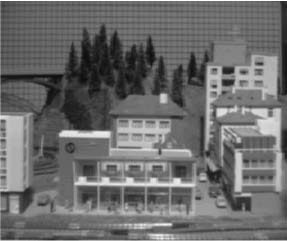
\includegraphics[width=\textwidth]{images/input.png}
    \caption{}
  \end{subfigure}
  ~
  \begin{subfigure}[b]{0.3\textwidth}
    \centering
    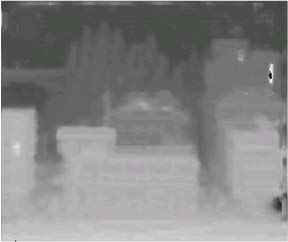
\includegraphics[width=\textwidth]{images/computed-depth.png}
    \caption{}
  \end{subfigure}
  ~
  \begin{subfigure}[b]{0.3\textwidth}
    \centering
    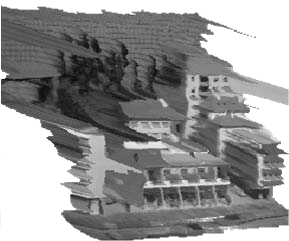
\includegraphics[width=\textwidth]{images/synthesized-view.png}
    \caption{}
  \end{subfigure}

  % newline

  \begin{subfigure}[b]{0.24\textwidth}
    \centering
    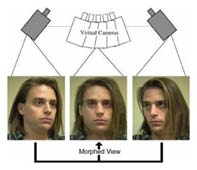
\includegraphics[width=\textwidth]{images/three-view.png}
    \caption{}
  \end{subfigure}
  ~
  \begin{subfigure}[b]{0.2\textwidth}
    \centering
    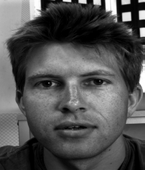
\includegraphics[width=\textwidth]{images/input-face.png}
    \caption{}
  \end{subfigure}
  ~
  \begin{subfigure}[b]{0.2\textwidth}
    \centering
    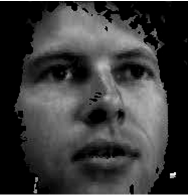
\includegraphics[width=\textwidth]{images/synthesized-face.png}
    \caption{}
  \end{subfigure}
  ~
  \begin{subfigure}[b]{0.2\textwidth}
    \centering
    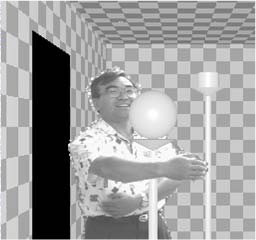
\includegraphics[width=\textwidth]{images/z-key.png}
    \caption{}
  \end{subfigure}

  % newline

  \begin{subfigure}[b]{0.3\textwidth}
    \centering
    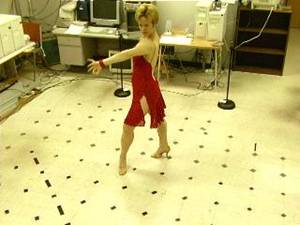
\includegraphics[width=\textwidth]{images/3d-input-left.png}
    \caption{}
  \end{subfigure}
  ~
  \begin{subfigure}[b]{0.3\textwidth}
    \centering
    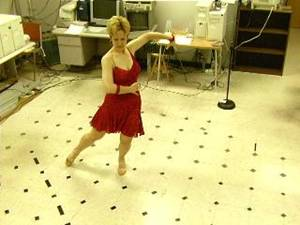
\includegraphics[width=\textwidth]{images/3d-input-right.png}
    \caption{}
  \end{subfigure}
  ~
  \begin{subfigure}[b]{0.3\textwidth}
    \centering
    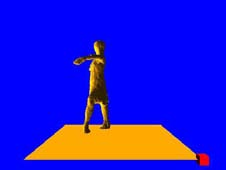
\includegraphics[width=\textwidth]{images/3d-reconstruction.png}
    \caption{}
  \end{subfigure}

  \caption{Applications of stereo vision: (a) input image, (b)
    computed depth map, and (c) new view generagtion from multi-view
    stereo \cite{matthies-kanade-szeliski}; (d) view morphing between
    two images \cite{seitz-dyer}; (e-f) 3D face modeling (images
    courtesy of Frederic Devernay); (g) z-keying live and
    computer-generated imagery \cite{kanade-yoshida-oda}; (h-j)
    building 3D surface models from multiple video streams in
    Virtualized Reality \cite{kanade-rander-narayanan}}
\end{figure}



\section{Problem Statement}\label{sect:prob-statement}

There are plenty of algorithms for disparity calculations. They all
have their characteristics; fast but coarse quality, good quality but
slow, good at object boundary but bad at continuous textureless areas.
These have all been researched heavily for decades, but has until
recently been very limited by the processing power of the days
computers. With the advent of cheap parallel computing devices in the
form of cheap consumer GPUs and cheap multi-cored CPUs, and frameworks
such as OpenCL and CUDA maturing, super-computer-like number crunching
has never been so fast and easy to do on home computers.

The goal of this thesis is to provide an implementation of the
algorithm most likely able to achieve real time estimation with High
Definition input.


\section{Main Contributions}\label{sect:contributions}

The main contribution of this thesis is a working OpenCL
implementation for GPUs able to run the depth estimation pipeline in
real time on high definition images. The evolution from a simple CPU
implementation to the final real time GPU implementation is documented
and analyzed, including many of the GPU architecture optimizations
approaches.

The secondary contribution is the \textit{compute mask} technique.
Sequential video frames contain a lot of redundant information. This
is especially true for statically mounted cameras filming some scene,
i.eg a theater stage. In such a scenario, the only moving objects in
the frames will often be just an actor or two, making the calculation
of the background redundant since it will result in the same value as
in the previous frame. The compute mask is a binary map indicating
whether a pixel needs to be calculated, or if the disparity value can
be copied from the disparity map of the previous frame.

\section{Limitations}\label{sect:limitations}

\subsubsection{Discretized disparity space}

The implementation produces 8-bit single channel gray-scale disparity
maps of the same dimensions as the input, which limits the number of
disparity levels to 256. This level of quantization may be fine for
some applications, like robotic navigation, but can lead to
unappealing results for other applications, like image-based view
synthesis.

\subsubsection{Camera calibration and Stereo rectification}

Input images must be stereo rectified. For a block matching algorithm
to be as effective as possible, it has to be able to assume that
corresponding points lie along the horizontal scan-line
(x-axis). Stereo rectification and camera calibration is such a
well-understood topic in computer vision, that most stereo
correspondence algorithms assumes its cameras are calibrated and the
inputs are rectified. 

\begin{figure}

  \begin{subfigure}[b]{0.48\textwidth}
    \centering
    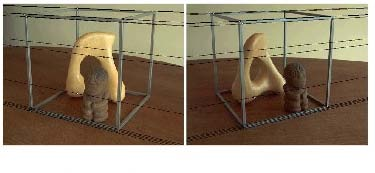
\includegraphics[width=\textwidth]{images/rectification-example.png}
    \caption{}
  \end{subfigure}
  ~
  \begin{subfigure}[b]{0.48\textwidth}
    \centering
    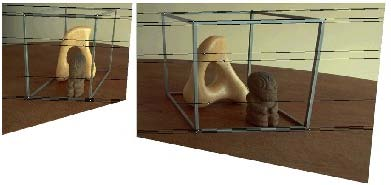
\includegraphics[width=\textwidth]{images/rectification-example-2.png}
    \caption{}
  \end{subfigure}

  \begin{subfigure}[b]{0.48\textwidth}
    \centering
    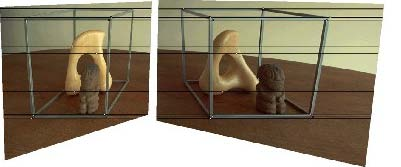
\includegraphics[width=\textwidth]{images/rectification-example-3.png}
    \caption{}
  \end{subfigure}
  ~
  \begin{subfigure}[b]{0.48\textwidth}
    \centering
    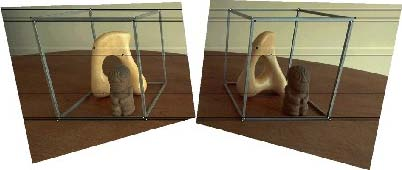
\includegraphics[width=\textwidth]{images/rectification-example-4.png}
    \caption{}
  \end{subfigure}

  \caption{An example showing various stages of Loop and
    Zhangs\cite{loop-zhang} proposed rectification algorithm. (a)
    Original image pair overlaid with several epipolar lines; (b)
    Image pair transformed so that epipolar lines are parallel to each
    other in each image; (c) Rectified image pair; (d) Final shearing
    transformation}

\end{figure}

To convert the disparity values to depth values, the intrinsic and
extrinsic matrices from the cameras that took the input images must be
provided. More specifically, the baseline (distance between the two
cameras) and the lenses focal length is needed in a formula, as will
be explained in chapter \ref{chap:depthestimation_theory}.

\section{Outline}

Chapter \ref{chap:depthestimation_theory} presents the core ideas of
stereo depth estimation in computer vision, and related work done in
the field. The OpenCL framework is presented in chapter
\ref{chap:arch}, along with some optimization strategies for GPU
devices. Chapter \ref{chap:impl} presents the code that has been
implemented. It starts off with the most basic depth estimator CPU
implementation, followed by an as direct as possible port to OpenCL.
From there, various optimizations are applied, followed finally by the
refinement kernels.

Lastly, chapter \ref{chap:eval} evaluates the results. It shows the
improvements most optimizations are able to bring, as well as the
quality of the depth maps using the different methods presented in
\ref{chap:depthestimation_theory}.

\chapter{Depth Estimation}
\label{sec:depthestimation_theory}


In this chapter we look at some of the core principals of depth
estimation theory, and some of the previous work done in the field.

\section{Introduction}

Extracting depth from images has been a heavily researched area of
computer vision for decades. As a result, there are many vastly
different techniques. But common for all the techniques are the

In short, depth estimation is about finding points in a 3D scene that
can be identified in two images taken from different points of
view. For each point, the difference in a points pixel coordinates in
one view relative to the other view, gives us the points disparity.

By finding the disparity of each point that is visible in both images,
we get a disparity map. With these disparity values, we can roughly
calculate the physical distance to these points from the cameras.

A simple demonstration of how two views viewing the same scene
changes; hold a finger vertically in front of your eyes. Close one of
your eyes alternatively, and notice how the fingers position changes
relative to the background. This change of position between the view
is the disparity. With some triangulation, the depth can be estimated.

\begin{figure}
  \label{fig:depth-theory}
  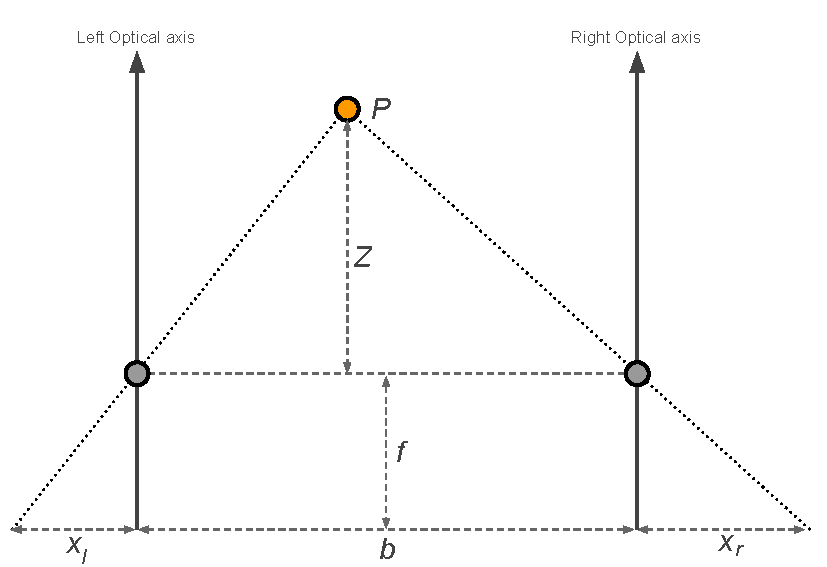
\includegraphics[width=\textwidth]{images/depth-estimation-theory.pdf}
  \caption{Example of how the depth can be calculated}
\end{figure}

Figure \ref{fig:depth-theory} shows how the depth \textit{Z} can be
triangulated. Finding the disparities \textit{Xl} and
\textit{Xr} is the main difficulty.


\section{Related Work}

Scharstein and Szeliski presents a very thorough taxonomy and
evaluation of some of the most known stereo correspondence algorithms
in \cite{taxonomy}. Most algorithms can be grouped into 3 distinct
sets:

\begin{itemize}
\item Feature-based
\item Graph cuts
\item Correlation based
\end{itemize}




\section{Depth Estimation Algorithms}

It is observed that most algorithms generally perform the following
four steps (or subsets of) \cite{taxonomy} :

\begin{enumerate}
\item Matching Cost computation
\item Cost (support) aggregation
\item Disparity computation/optimization
\item Disparity refinement
\end{enumerate}

Most stereo algorithms can be grouped into two main categories;
\textit{local} and \textit{global} algorithms.

Local algorithms estimate depth with the help of its neighboring
pixels only. This neighborhood varies between algorithms, but is most
often a square window of $7\times7$ to $21\times21$ pixels. Other
local algorithms may use adaptive windows that changes shape on
certain conditions, or non-square shapes.

Global algorithms make explicit smoothness assumptions and then solve
an optimization problem. This thesis will not cover global algorithms.

\subsection{Matching Cost calculation}
\label{sec:matchingcost}

The matching cost is a measurement of the similarity of pixel
locations in the input images. This calculation is typically done for
all pixels, at all the disparity hypotheses.

There are many ways to calculate this. Two of the simplest methods are
\textit{Absolute intensity differences} (AD) and \textit{Squared
  intensity differences} (SD). These methods are very computationally
quick to calculate, AD even more so than SD.


\begin{figure}
  \label{eq:sad}
  \[ \mathlarger{\mathlarger{\sum}}_{i,j \in w} |I_L(i,j) - I_R(x + i, y + j)| \]
  \caption{Sum of Absolute intensity Differences}
\end{figure}


\begin{figure}
  \label{eq:ssd}
  \[ \mathlarger{\mathlarger{\sum}}_{i,j \in w} (I_L(i,j) - I_R(x + i, y + j))^2 \]
  \caption{Sum of Squared intensity Differences}
\end{figure}

A third well known technique is \textit{Birchfield and Tomasi}'s (BT)
image sampling insensitive method \cite{bt}. Instead of comparing
pixel values shifted by integral amounts, BT compares each pixel in
the reference image against a linearly interpolated function of the
other image.

\begin{equation}
  \label{eq:bt}
  \mathlarger{\mathlarger{\sum}}_{i,j \in w} d(x_L, x_R, I_L, I_R) = \max\{0, I_L(x_L) - I_{max}, I_{min} - I_L(x_L) \}
\end{equation}


A lower cost is a better match, where a cost of 0 means the left and
right pixels are identical.

\subsection{Aggregation of Costs}
\label{sec:aggregatecost}

Single pixel matching is in most cases too ambiguous. Some kind of
additional information is needed. For \textit{local} algorithms,
summing or averaging a small neighborhood of pixel-costs into an
aggregated cost yields a much better value for comparison.

The simplest way is to sum the costs in a window around the pixel of
interest. This method is known as \textit{Sum of Absolute Differences}
(SAD) or \textit{Sum of Squared Differences}, depending on which cost
matching was used.

Another slightly more complex technique is to use \textit{Adaptive
  Windows}\cite{Okutomi and Kanade, 1992; Kanade and Okutomi, 1994;
  Veksler, 2001; Kang et al., 2001)}. Figure \ref{fig:adaptivewindow}
demonstrates what an adaptive window looks like. Cost matching is done
normally with either AD or SD. Each square is then aggregated
separately. What gives this technique its name is which of the squares
are used as the final aggregation cost; it selects the two windows
with the lowest scores, and the center square. This method is better
along depth disparities, since windows spanning an occlusion is much
less likely to be included in the final selection.

A lower aggregated cost is a better match, where a cost of 0 means the
left and right pixels and its neighborhood are identical.

\subsection{Disparity Selection}
\label{sec:disparity_selection}

This step involves finding which disparity level has the best
match. The easiest way is to compare each cost at each disparity
level, and select the level with the lowest cost. This strategy is
called \textit{winner-takes-all} (WTA).




\subsection{Refinement}
\label{sec:refinement}

Most depth estimation algorithms produce a disparity map of integer
disparities. Many applications such as robotics navigation and
tracking are fine with that level of quantization. However, for
image-based rendering such as \textit{Visual Hulls} and
3D-reconstruction, this level is detail is detrimental to the quality
of their output. This can be alleviated by applying a sub-pixel
refinement stage. Linear interpolation may be too simple, but others
have researched methods like including an iterative gradient descent
and fitting a curve to the matching costs at discrete disparity levels
\cite{Ryan et al., 1980; Lucas and Kanade, 1981; Tian and Huhns, 1986;
  Matthies et al., 1989; Kanade and okutomi, 1994, taxonomy}.

Applying a median filter to the disparity map removes high-intensity
noise caused by erroneous and spurious matches. Along an objects
surface the disparity is most likely going to be continuous, and
blurring may even out slightly-off matches.

Cross-checking is a method that requires a disparity map for both the
left and right images.

Cross-checking eliminates unreliable matches. All depth
discontinuities will have occlusions, where a real world point is only
visible on one of the images, and will also always produce an
unreliable match.

When cross-checking and eliminating unreliable matches, holes of
uncalculable disparity are left in the disparity map. These holes can
be artificially filled with guesses; it is very likely that the
disparity in the occlusions are continuous

sub-pixel refining

\section{Summary}

Depth estimation is about

\chapter{GPU and OpenCL}
\label{chap:arch}
``OpenCL (Open Computing Language) is an open royalty-free standard
for general purpose parallel programming across CPUs, GPUs and other
processors, giving software developers portable and efficient access
to the power of these heterogeneous processing platforms''
\cite{cl-spec}

\section{Introduction}

In the 1980s, graphics processing units (GPU) began as coprocessors
assisting the central processing units (CPU) with graphics related
computations like drawing lines, arcs, rectangles. GPUs evolved from
these early graphics-oriented instruction sets, specializing in
manipulating and altering images. The parallel nature of graphics
processing, doing the same computations on multiple elements,
eventually led to GPUs with a highly parallel architecture.

General purpose computing on graphics processing units (GPGPU) are
GPUs that are able to perform calculations for applications typically
only run by central processing units (CPU). GPUs are high-performance
many-core processors specialized for compute-intensive and highly
parallel computations, capable of very high throughput. They are
designed with data processing in mind, compared to a CPU which is more
specialized in caching and flow control, as illustrated in figure
\ref{fig:cpu-vs-gpu}. The GPUs parallel throughput architecture
emphasizes executing many concurrent threads slowly, unlike the CPU
that aims to execute a single thread very quickly.

Earlier GPGPUs required the use of graphics programming APIs like
OpenGL and Cg, which limited the general purpose programming
capability tremendously. But in 2007, Nvidia released CUDA, a
proprietary GPGPU framework, which supports parallel programming on a
GPU in C, closely followed by OpenCL in 2008.

\begin{figure}
  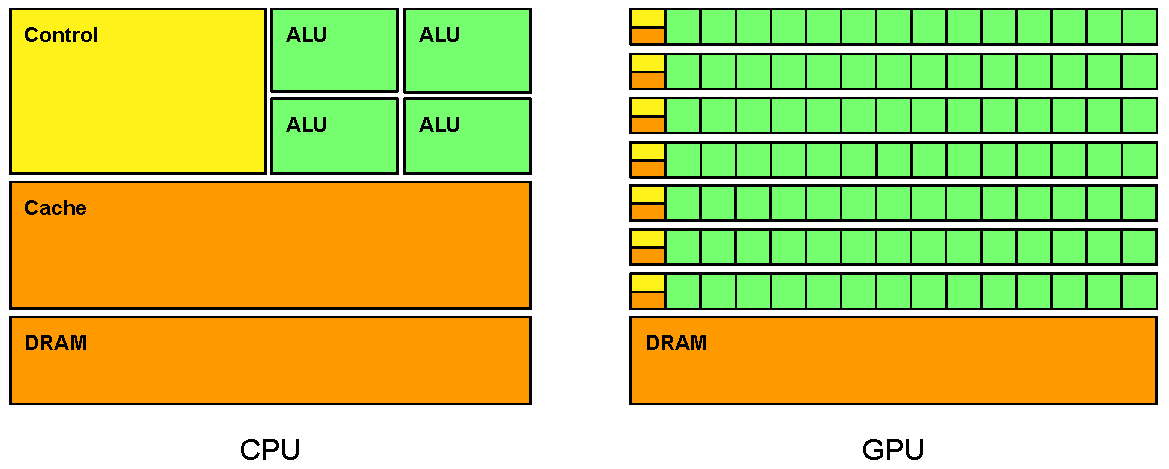
\includegraphics[width=0.8\textwidth]{images/cpu-vs-gpu.pdf}
  \caption{GPUs devote more transistors to data processing than CPUs}
  \label{fig:cpu-vs-gpu}
\end{figure}


\section{OpenCL}

OpenCL was initially proposed by Apple in 2008 and refined in
collaboration with teams from AMD, IBM, Intel and Nvidia. The initial
proposal was submitted to the Khronos Group\cite{cl-spec}, who later
that year released the first OpenCL specification.

The specification is designed as a framework for programming a
heterogeneous collection of CPUs, GPUs and other computing devices
organized into platforms. OpenCL provides low-level hardware
abstraction and an API that supports the underlying hardware to allow
for portable and efficient code. Being a specification and not a
technology in itself, OpenCL needs to be implemented by vendors who
wish to be able to run OpenCL applications and brand themselves OpenCL
compliant. The largest vendors of parallel computing devices have
implementations for OpenCL 1.1 on most operating systems, including
IBM's Power7\cite{ibm-opencl}, most of Nvidias
GPUs\cite{nvidia-opencl}, most of AMDs CPUs and GPUs \cite{amd-opencl}
and Intels CPUs \cite{intel-opencl}.

As frameworks, OpenCL is very similar to Nvidias Compute Unified
Device Architecture (CUDA), but very unlike other parallel computing
frameworks like Hadoop\cite{hadoop} and OpenMP\cite{openmp}. CUDA
currently only works on Nvidia GPUs, while OpenCL currently supports a
number of GPUs, CPUs, DSPs and a number of other accelerator devices.
Additionally, OpenCL also supports task-parallelism, which means
[TODO: describe!]

\subsection{The OpenCL Specification}

The core ideas behind OpenCL are described in a hierarchy of four
models\cite{cl-spec}:

\begin{enumerate}
  \item Platform model
  \item Execution model
  \item Memory model
  \item Programming model
\end{enumerate}

This section contains a condensed summary of the OpenCL specification
without going to in-depth, just to give a basic understanding of how
it works.

\vspace{5mm} \textbf{Device}:


% \vspace{10mm}
% \textbf{Platform model}:
\subsubsection{Platform model}

``An OpenCL Platform is defined as a host connected to one or more
OpenCL devices. An OpenCL device is divided into one or more compute
units which are further divided into one or more processing elements.
Computations on a device occur within the processing elements.''
\cite{cl-spec}

\begin{figure}
  \centering
  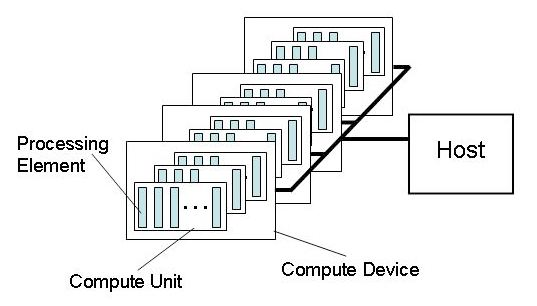
\includegraphics[width=0.8\textwidth]{images/platform-model.png}
  \caption{Platform model, one host plus one or more compute devices,
    each with one or more compute units, each with one or more
    processing elements}
  \label{platform-model-figure}
\end{figure}

An OpenCL device is a collection of compute units. Any processor that
conforms to the OpenCL specification can be a device, ranging from
GPUs, CPUs to DSPs and Cell Broadband Engine processors. A compute
unit is an abstraction for the number or cores the processor has.

A typical home computer usually contains 2 OpenCL compatible devices;
a multi-core CPU and a GPU. Most vendors of consumer CPUs and GPUs
(Intel, AMD, ATI and Nvidia) have OpenCL implementations for their
respective devices available for Linux, OSX and Windows.

The machine used to benchmark the implementation in this thesis, an
Intel i7 CPU and an Nvidia GTX 460, forms 2 platforms. Both Intel and
Nvidia provides an OpenCL implementation for the CPU and the GPU
respectively, and can both be used as OpenCL devices. The host for
both platforms is the CPU device.

% \vspace{10mm}
% \textbf{Execution model}:
\subsubsection{Execution model}

``Execution of an OpenCL program occurs in two parts: kernels that
execute on one or more OpenCL devices and a host program that executes
on the host. The host program defines the context for the kernels and
manages their execution.'' \cite{cl-spec}

When a kernel is submitted for execution, the host defines an index
space. Each point in this index space will be executed by an instance
of the kernel. The index space is called an N-Dimensional Range, or
NDRange, where N can be 1, 2 or 3, and is defined as an N dimensional
integer array. The length of each dimension defines how many
work-items will be launched. The NDRange is often mapped to the
dimensions of either the input or output data.

Work-items can be identified by its coordinates in the index space,
called a global ID. Work-items are further organized into work-groups,
which provides a more coarse grained decomposition of the NDRange.
Work-groups are also uniquely identifiable with a work-group ID.
Work-items in a work-group are assigned a unique ID local to that
work-group. Work-items within a work-group execute concurrently on the
processing elements of a single compute unit.

Figure \ref{execution-model-figure} shows a 2-dimensional NDRange of
$G_x \times G_y$ work-items, organized into $W_x \times W_y$
work-groups, each having $S_x \times S_y$ work-items. A work-item can
be identified multiple ways; by its global ID, by a combination of the
work-group size and ID and the work-items local ID.

\begin{figure}[h]
  \centering
  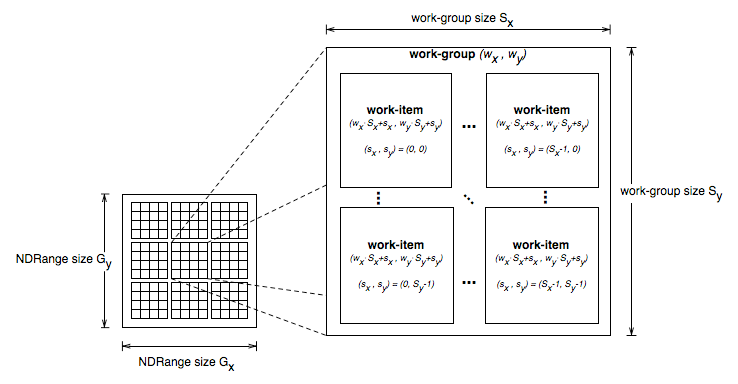
\includegraphics[width=0.8\textwidth]{images/execution-model.png}
  \caption{An example of an NDRange index space showing work-items,
    their global IDs and their mapping onto the pair of work-group and
    local IDs}
  \label{execution-model-figure}
\end{figure}


% \vspace{10mm}
% \textbf{Memory model}:
\subsubsection{Memory model}


``Defines the abstract memory hierarchy that kernels use, regardless of
the actual underlying memory architecture. The memory model closely
resembles current GPU memory hierarchies, although this has not
limited adoptability by other accelerators.''

The memory model specifies 4 distinct memory regions that a work-item
has access to:

\begin{itemize}
\item \textbf{Global Memory}: Similar to the main memory of a desktop
  computer. This memory is visible for all work-items, and is the main
  storage space for kernels input and output data.

\item \textbf{Constant Memory}: This memory is intended for values
  which don't change during execution, and is likely needed by all
  work-items simultaneously during execution. Constant like $\pi$,
  look-up tables of $\sin$ and $\cos$ values, etc. The memory is
  read only, and visible for all work-items.

\item \textbf{Local Memory}: This memory is shared by all work-items
  in the same work-group, with read and write access. It is a
  scratchpad memory, commonly implemented in devices as on-chip memory,
  providing low latency and high bandwidth but at a limited amount.

\item \textbf{Private Memory}: Private memory is unique for each
  work-item, used to store local variables and non-pointer kernel
  arguments.

\end{itemize}

How each of these memory types are implemented is up the vendors. For
GPUs, each of these memory types corresponds to physical memories on
most device. Global memory is mapped to the cards DRAM, constant
memory to a cached region of the DRAM, local memory to the cache on
each multiprocessor, and private memory to the cores registers.

\begin{figure}[h]
  \centering
  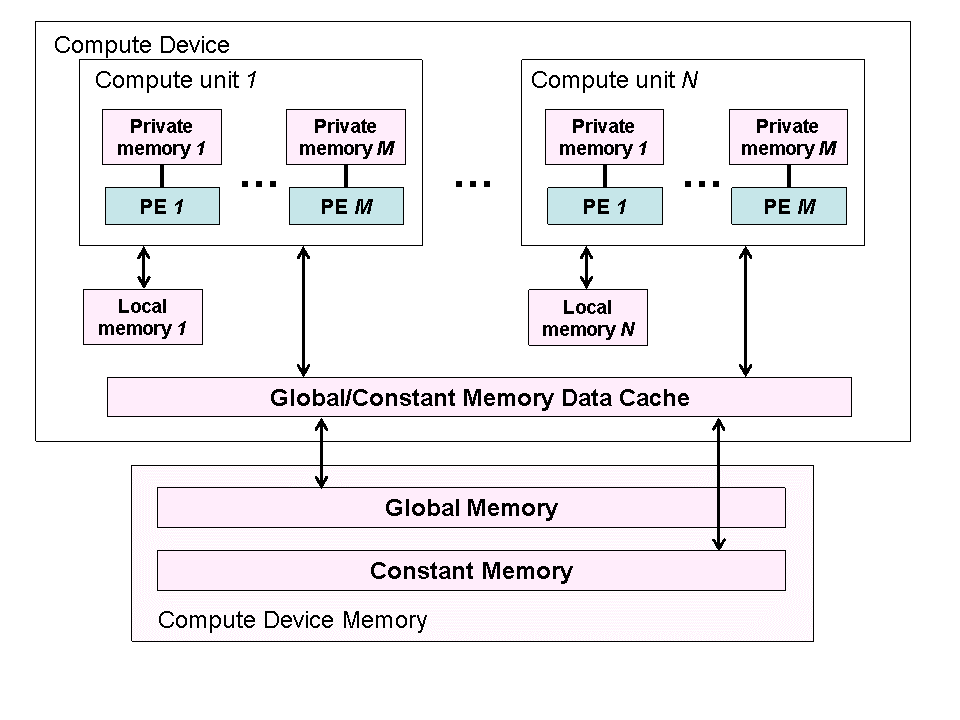
\includegraphics[width=0.8\textwidth]{images/memory-model.png}
  \caption{Conceptual OpenCL device architecture with processing
    elements (PE), compute units and devices. The host is not shown.}
  \label{execution-model-figure}
\end{figure}



% \vspace{10mm}
% \textbf{Programming model}:
\subsubsection{Programming model}

``Defines how the concurrency model is mapped to physical hardware.''

OpenCLs execution model supports both data parallel and task parallel
programming models. The data parallel programming model defines a
computation in terms of a sequence of instruction applied to multiple
elements of a memory object. The NDRange from the execution model
defines how many work-items are used, and how it is mapped to the
data.


\subsection{Kernels}

An OpenCL kernel is a kind of function written in OpenCL-C that is
executed by an OpenCL capable device. OpenCL-C is based on C99, with
some restrictions and added extensions. The most noticeable
restrictions include no recursion and no function pointers. The
extensions include new vector data types like int4 and float4 etc, and
2D and 3D image types.



\section{GPU Optimization Strategies}

There are many considerations that need to be taken into account when
programming for efficiency on a GPU. Although OpenCL programs are
portable, the same application might not be as effective on a CPU as
it is on a GPU. This section will explain some of the optimization
strategies useful for the Nvidia GPU used in this thesis, with a focus
on the ones implemented in chapter \ref{eval-chapter}. More
information is available online from Nvidias Best Practice
article\cite{nvidia-best-practice}.



\begin{itemize}

\item \textbf{Memory optimizations}: a GPUs memory is divided into different
  types, with different properties and sizes, so choosing the best
  memory type for the job is important.

\item \textbf{NDRanges optimizations}: Choosing the best work-group
  sizes to utilize as much of the multiprocessors resources.

\item \textbf{Instruction optimizations}: Some instructions use fewer
  clock cycles than others.

\item \textbf{Control flow}: Execution branching can force the GPU to
  execute parallel code serially, so careful thought and organization
  is important.

\end{itemize}

These strategies applies 

\subsection{Memory Optimizations}

Effectively using the GPUs memory correctly can net large performance
gains. OpenCLs memory model closely resembles current GPUs memory
hierarchy (as shown in \ref{fig:memory-model-figure}), and include
\textit{global}, \textit{local}, \textit{shared}, \textit{texture},
\textit{registers}, \textit{constant} and \textit{texture}. Table
\ref{table:memory-properties} lists the properties of each memory
space.

\begin{table}
  \begin{tabular}{|l|l|l|l|l|l|}
    \hline
    Memory Space & Location on/off chip & Cached & Access & Scope                & Lifetime        \\ \hline
    Register     & on                   & n/a    & r/w    & 1 thread             & thread          \\
    Local        & off                  & no     & r/w    & 1 thread             & thread          \\
    Shared       & on                   & n/a    & r/w    & all threads in block & block           \\
    Global       & off                  & no     & r/w    & all threads and host & host allocation \\
    Constant     & off                  & yes    & r      & all threads and host & host allocation \\
    Texture      & off                  & yes    & r      & all threads and host & host allocation \\
    \hline
  \end{tabular}
  \label{table:memory-properties}
  \caption{List of the Nvidia GeForce 460 GTX memory spaces on the and their properties}
\end{table}

The simplest implementations can use global memory exclusively. But,
accessing global memory on a GPU is by far the slowest operation
available, so reading and writing to it without a care will work, but
impacts the performance. Smart use of all the memory spaces will
increase performance significantly. Constant memory can be used for
look-up tables and constant values, local memory for sharing data
between work-items, texture memory to exploit the cache, and so on. 

\subsubsection{Global Memory Access Patterns}
\label{sect:global-memory-optimization}
One of the most important performance considerations is how this
global memory is accessed. Each store and load operation to the memory
is done by half warps (16 threads), coalesced in as few as one
transaction, in 32-, 64- or 128-byte segments. The exact number of
threads and the segment sizes depends on the GPU and the data type,
and newer GPUs with higher compute capability\ref{what-is-cc?} are
more lenient on how each data segment is laid out, but the general
principle is that few transactions can transfer a lot of data.

\begin{figure}[h]
  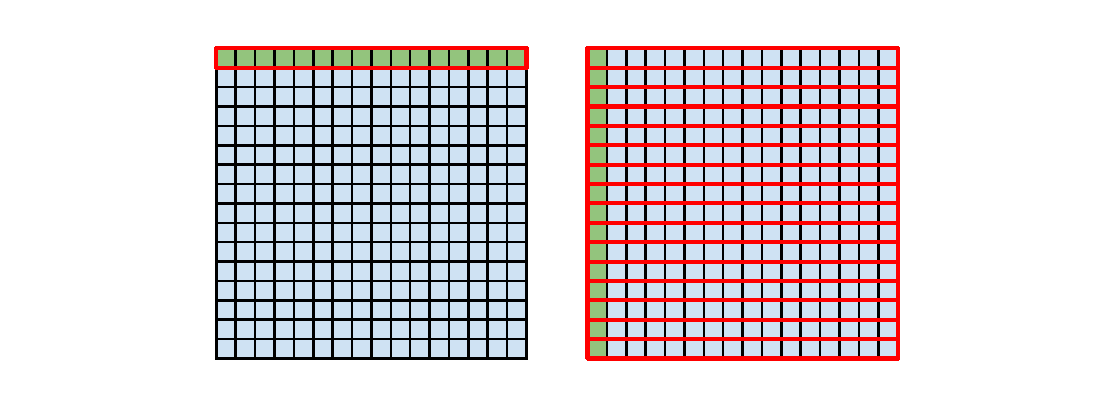
\includegraphics[width=\textwidth]{images/coalesced-access.pdf}
  \caption{Grossly simplified demonstration of how sequential data
    (left group) can be accessed in 1 transaction by a half warp,
    while strided data (right group) results in 16 transactions, where
    only 1 block of data from each read is used.}
  \label{fig:execution-model-figure}
\end{figure}

As seen in figure \ref{fig:execution-model-figure}, laying out the
data needed by the application correctly can increase the bandwidth on
memory transfers greatly.

\begin{lstlisting}[label={lst:coalesced_test}, caption=Copy kernel
  with offset argument]
  __kernel void offsetCopy(__global float *odata,
                           __global float* idata,
                           int offset)
  {
    int xid = get_global_id(0) + offset;
    odata[xid] = idata[xid];
  }
\end{lstlisting}

Misaligned data accesses can be demonstrated with the simple copy
kernel listed in \ref{lst:coalesced_test}. This kernel is launched 32
times with the offset parameter incremented by 1 for each kernel.
Figure \ref{fig:coalesced-performance} shows measurements for 2 Nvidia
devices; GeForce GTX 280 with compute capability 1.3 and GeForce GTX
8800 with compute capability 1.0.

\begin{figure}[h]
  \centering
  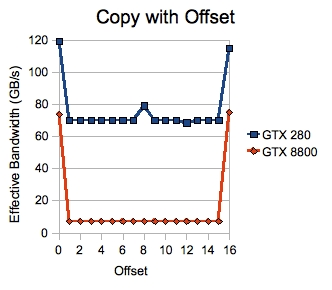
\includegraphics[width=0.5\textwidth]{images/coalesced-performance.png}
  \caption{Performance decrease with misaligned accesses}
  \label{fig:coalesced-performance}
\end{figure}

With offset that are multiples of 16, accesses can be done with 1
transaction per half-warp for the highest bandwidth possible.
Otherwise, 16 transactions per half-warp are issued, resulting in a
performance degradation of at least 8x, because 32 bytes are fetched
per access, but only 4 bytes of those reads are kept.

\subsubsection{Local memory}
\label{sect:local-mem-optimization}

The OpenCL Local memory space is mapped to the GPUs on-chip shared
memory, which provides very low latency and very high throughput
compared to the global memory. There is however a very limited size,
and very rigid rules to follow in order to achieve the maximum
performance.

The memory is divided into memory banks of equal size that can be
accessed simultaneously by threads in the same work-group.

\subsection{NDRange optimizations}
\label{sect:ndrange-optimization}



\subsection{Instruction optimizations}
\label{sect:instruction-optimization}

\subsection{Control flow}
\label{sect:control-flow}

\section{Depth Estimation on a Parallel Architecture}

This architecture fits the problem of estimating depth perfectly.
Estimating depth is a very data-parallel task, meaning that each pixel
in the resulting depth map can be calculated independent of the other
pixels, in parallel.

An example of a non-data-parallel task is summing up the values in an
array. This is a sequential task, in that each addition of values is
dependent on the previous addition. It is possible to parallelize this
task, but its nature is not data-parallel. For this task, using more
cores to will not increase the performance.

Box filtering is an easy to understand example of a data-parallel
task. The algorithm for the filter is basically; each pixel in the
original image is written into a new image as an average of that
pixels surrounding pixels.

In depth estimation, block matching algorithms have a similar nature
to that of box filtering; each output pixel can be processed
completely on its own. More cores means more tasks can be scheduled in
parallel.

As we'll see in chapter \ref{eval-chapter}, the performance increase
is formidable.

\chapter{Implementation}

\section{The Algorithm}

Several depth estimation algorithms have been described in section
\ref{sec:depthestimation_theory}. A block matching algorithm
\texttt{[TODO: reference to some paper. Other than the taxonomy, for
  some variation!]} was chosen due to it's simplicity, decent quality
and speed. Since it is a local algorithm \texttt{[TODO: reference the
  taxonomy paper]}, it is very data parallel and well suited for the
GPU architecture.

The algorithm can be viewed as a pipeline containing the rough steps:

\begin{enumerate}
\item Correlation cost
\item Aggregation of costs
\item Disparity selection
\item Refinement and post-processing
\end{enumerate}

This chapter will present basic and optimized versions of each of
these steps, and a short conclusion for why a version was chosen for
the final real time algorithm.

\section{Overview}

The block matching algorithm has an O(1) complexity. But for HD input,
the amount of calculations is still large enough for it to not run in
real time, unless heavy optimizations are applied.

A simple version of a block matching algorithm would have to calculate
the pipeline for $H \times W \times D$ pixels. For an algorithm with
an $N \times N$ aggregation window, the number of calculations for a
pipeline would be $N \times N \times 3$. In total, $H \times W \times
D \times N \times N \times 3$. For a $1024 \times 768$ image, $9
\times 9$ aggregation window and $255$ disparity search range,
calculations are needed. For stereo depth maps, twice that is needed.
And for real tdsime (25 fps) videos, multiply that with 40.


\subsection{Assumptions}

The input images need to be stereo rectified single channel 8-bit
grayscale.

For the diffing to be effective, the camera rig and scene should be
stationary. Less foreground objects moving on the scene will result in
faster run times.

No non-Lambertian surfaces. That is, the surface needs to reflect the
same apparent brightness from all perspectives. Will result in
matching errors.

Note: All code listings are simplified. Boundry checks, variable
declarations and function signatures are mostly excluded.
\texttt{[TODO: Should the code listings be simplified?]}

\section{CPU Implementation}

The CPU implementation is a proof-of-concept, rather than a usable
prototype, to set the bar for a serious GPU implementation. It is
possible to heavily optimize it, but it will most likely never reach
real time on current commodity hardware. It was made to clearly
outline what a block matching algorithm really does, and to be able to
identify data dependencies, potential parallelization and data sharing
problems that the GPU versions must deal with intelligently.

This version calculates all the pipeline steps separately, storing
temporary calculations in memory between the steps. It uses SSD or SAD
for matching costs and WTA disparity selection strategy. It only
calculates a depth map for the left input image, and there is no
refinement step.

Listing \ref{lst:CPU_implementation} shows the core functions of the
algorithm. After initialization of buffers and input parameters, they
are called in the order marked by the comment. After the last function
returns, the disparity map is complete.

%% It was implemented like this with the hope of being able to optimize
%% each step separately, and to be able to quickly swap out different
%% version of the steps cleanly. Many problems with this approach was
%% discovered later in the development, after implementing the initial
%% GPU version. Because the main focus is on the GPU implementation,
%% these problems were not fixed in the CPU implementation.

%% The main depth estimation function takes 4 arguments: two stereo
%% rectified 8-bit gray-scale images, and two allocated 8-bit disparity
%% map buffers of the same size as the input images. You can also set the
%% settings: maximum disparity, aggregation window size.

%% It then initializes the needed buffers, and calls the functions listed
%% in listing \ref{lst:CPU_implementation}.

\begin{lstlisting}[label={lst:CPU_implementation}, caption=CPU
  implementation of the 3 first steps in the pipeline]

  // (1)
  void calculateCosts() {

    /* For each pixel, go through each disparity level and calculate
    the cost, and store it in a costs array */

    for(int y = 0; y < HEIGHT; y++) {
      for(int x = 0; x < WIDTH; x++) {
        for(int d = 0; d < MAX_DISP; d++) {
          int index = y * HEIGHT + x;
          int cost = abs(left[index] - right[index - d]);
          costs[(d * HEIGHT * WIDTH) + (y * WIDTH + x)] = cost;
        }
      }
    }
  }

  // (2)
  void aggregateCosts() {

    /* The radius of the aggregation window */
    int r = AGGREGATION_WINDOW_SIZE/2;

    /* For each cost, add up the costs of the neighboring
    pixels in a r of AGGREGATION_WINDOW_SIZE */
    for(int y = r; y < HEIGHT - r); y++) {
      for(int x = r; x < WIDTH - r); x++) {
        for(int d = 1; d < MAX_DISP; d++) {
          /* Now we need to iterate over the pixels that
          form a window around the current pixel of
          interest */
          int sum = 0;
          for(int i = y - r; i <= y + r; i++) {
            for(int j = x - r; j <= x + r; j++) {
              sum += costs[i * WIDTH + j];
            }
          }
          aggregated_costs[d * HEIGHT * WIDTH + (y * WIDTH + x)] = sum;
        }
      }
    }
  }

  // (3)
  void disparitySelection() {

    int best_match = MAX_INTEGER;
    int best_disparity = 0;

    for(int y = 0; y < HEIGHT; y++) {
      for(int x = 0; x < WIDTH; x++) {
        int pixel = y * WIDTH + x;
        for(int d = 0; d < MAX_DISP; d++) {
          if(aggregated_costs[IMG_SIZE * d + pixel] < best_match) {
            best_match = aggregated_costs[IMG_SIZE * d + pixel_index];
            best_disparity = d;
          }
        }
        disparity_map[pixel] = best_disparity;
      }
    }
  }
\end{lstlisting}

This code marked by (1) shows step 1 in the pipeline, calculating the
cost of all the pixels at all the disparity levels, and stores it in a
costs array. This array needs to be of size \begin{math} (H \times
  W)D \end{math} bytes.

The next step is aggregating costs in a window of a chosen size. This
window's dimension has a default value of 9 pixels, which is an all
around good value for both quality and speed. The code marked by (2)
shows how this is done. This is the most computation heavy step in the
pipeline.

The next step is to select the best match and what disparity level
this was found at. In all implementations, WTA was chosen because of
its simplicity and quality compared to the other methods mentioned in
\texttt{[TODO: reference related work section]}. WTA is basically just
a straightforward search through unordered MAX\_DISP integers. The
biggest difference between WTA implementations is how to handle
multiple best matches. It can either keep the first best match, or the
latest best match. Either way, it will most likely result in a
matching error, which can only be solved in the cost calculation or
aggregation step in the pipeline. The code marked by (3) shows a
simple version with keeping the first best match. To keep the last
best match, just replace the less than with less than or equal.

This step completes the CPU implementation of the algorithm.


\section{GPU Implementation}

The GPU implementation is implemented using OpenCL, running on an
Nvidia GeForce 460 GTX, a cheap off the shelf graphics card.

\subsection{Initial implementation}

The first implementation was an attempt at a 1:1 port of the CPU
implementation, with a kernel for each step in the pipeline. The host
first transfers the input buffers and allocates the output buffers on
the device's global memory. Then

These
kernel functions are then queued to process th one after the other, storing their
intermediate results to global memory, until all pixels have been
processed.

\begin{lstlisting}[label=calculateCosts,caption=Matching Cost kernel]
  /* Kernel to calculate the costs of each pixel at each disparity
  levels, storing the results to global memory */
  __kernel void calculateCost(...) {
    int2 gid = (int2)(get_global_id(0), get_global_id(1));
    int left_pixel = left_img[gid.y * WIDTH + gid.x];
    for(int d = 0; d < MAX_DISP; d++) {
      int cost = abs(pixel - right_img[gid.x * WIDTH + gid.x - d]);
      costs[gid.y * WIDTH + gid.x + d * IMG_SIZE] = cost;
    }
  }
\end{lstlisting}


\begin{lstlisting}[label=aggregateCosts,caption=Cost aggregation kernel]
  __kernel void aggregateCosts(...) {

    /* The radius of the aggregation window */
    int radius = AGGREGATION_WINDOW_SIZE/2;

    int2 gid = (int2)(get_global_id(0), get_global_id(1));

    int  sum = 0;
    for(int d = 0; d < MAX_DISP; d++) {
      for(int y = 0; y < AGGREGATION_WINDOW_SIZE; y++) {
        for(int x = 0; x < AGGREGATION_WINDOW_SIZE; x++) {
          [TODO: finish this code]
        }
      }
    }
  }
\end{lstlisting}


\begin{lstlisting}[label=disparitySelection, caption=Disparity
  selection kernel]

  TODO: Write this code!

\end{lstlisting}


\texttt{[TODO: Re-implement this first version, and show run-times]}

This first version works much faster than the CPU version, but it is
nowhere near real time. The memory usage is also too high for
HD-inputs with reasonable disparity search ranges. The temporary
values calculated by step 1 in the pipeline ends up at $ W \times H
\times D $ bytes. For HD-images with a max search range of 256 pixels,
these cost values add up to 235 mb. The aggregation step also needs an
equally large array to store the aggregated costs. Even though the
GeForce 460 GTX has 1 gb global memory, the largest possible memory
allocations are 200 mb regions at a time, which makes implementing
this for HD-images even more impractical.

So one of the first things to tune had to be to lower the memory
usage.

\subsection{Reduce memory usage}

Because the pipeline steps were implemented seperately, every cost
calculation and aggregated cost had to be stored so they could be used
by the next step in the pipeline. But they are really just temporary
values. Each pixel only needs to know about the costs around itself,
so instead of separate kernels for each step, implementing a kernel
that calculates all the steps by istelf removes the need to store
everything in global memory. There will be an increase in redundant
cost calculations, but the overall performance will also increase
because of the reduced overhead of reading and writing huge result
buffers between the pipeline steps.


\begin{lstlisting}[label={lst:calculatedisparity},caption=Single kernel to
  calculate the whole pipeline]
  __kernel void calculateDisparity(...) {

    const int x = get_global_id(0), y = get_global_id(1);
    const int offset_x = x - window_dim/2;
    const int offset_y = y - window_dim/2;

    if(offset_x >= 0 && offset_x + window_dim < width) {
      unsigned int sum = 0, best_sum = -1, best_d = 0;
      for(int d = 0; d < max_disp; d++) {
        for(int i = offset_y; i < window_dim + offset_y; i++) {
          for(int j = offset_x; j < window_dim + offset_x; j++) {
            sum += abs((int)img_l[i * width + j] -
            (int)img_r[i * width + j - d]);
          }
        }
        if(sum < best_sum) {
          best_sum = sum;
          best_d = d;
        }
        sum = 0;
      }
      result[y*width+x] = best_d;
    }
  }
\end{lstlisting}

Listing \ref{lst:calculatedisparity} shows a single kernel that
calculates the whole pipeline. Each work-item's global ID specifies
which pixel it is working on. It first calculates the SAD or SSD of
the aggregation window surrounding the pixel, then checks if this
disparity level is the best match (or equally good, depending on the
disparity selection strategy). The best match so far is kept, and it
continues the loop. Finally, the disparity level containing the
selected best match is written to the depth map.

This version avoids the need to store any of the temporary values the
other version needed, and cut the memory usage from > 800MB to just 2
input images and 2 disparity maps, that is, 4 * IMAGE\_SIZE bytes.

\subsection{Using Local memory}

The next optimization is to use local memory to cache the pixels that
each work-group knows it will be needing. Because each work-item is
working independently on calculating it's own disparity value, many of
the same input pixels are accessed multiple times by adjacent
work-items.

Accessing global memory is much more costly than local memory
accesses, and should be minimized as much as possible, as explained in
section \ref{sect:optimize-memory}. It's easy to see which pixels all
the work-items in a work-group will be needing access to, as seen in
figure \texttt{[TODO: create and reference a figure! Similar to the
  one used in the presentation]}.

The code in listing \ref{lst:local_memory_code} reduce the number of
global accesses from \texttt{[TODO: do some math on this]} to only one
read per pixel.

\begin{lstlisting}[label={lst:local_memory_code}, caption=Using
  local memory to reduce the number of global memory accesses]

  /* fill the left local memory buffer */
  for(i = 0; i < local_height; i += get_local_size(1)) {
    for(j = 0; j < local_width; j += get_local_size(0)) {
      local_left[(lid.y + i) * local_width + (lid.x + j)] =
      img_l[((gid.y - AGGR_RADIUS + i) * PADDED_WIDTH) + gid.x - AGGR_RADIUS + j];

      local_right[(lid.y + i) * local_width + (lid.x + j)] =
      img_r[((gid.y - AGGR_RADIUS + i) * PADDED_WIDTH) + gid.x - AGGR_RADIUS + j - MAX_DISP];
    }
  }

  barrier(CLK_LOCAL_MEM_FENCE);

  /* calculate the disparities */
  for(d = 0; d < MAX_DISP; d++) {
    for(i = 0; i < AGGR_DIM; i++) {
      for(j = 0; j < AGGR_DIM; j++) {
        current_left_sum += abs(local_left[((lid.y+i) * local_width) + lid.x + j] -
        local_right[((lid.y+i) * local_width) + lid.x + j - d + MAX_DISP]);

        /* current_right_sum += abs(local_right[((lid.y+i) * local_width) + lid.x + j + MAX_DISP] - */
        /*                          local_left[((lid.y+i) * local_width) + lid.x + j + d]); */
      }
    }

    if(current_left_sum < best_left_sum) {
      best_left_sum = current_left_sum;
      best_left_disparity = d;
    }
    current_left_sum = 0;
  }
\end{lstlisting}

\texttt{[TODO: This code listing is just copy-pasted. Needs to be
  edited/simplified a bit]}


\subsection{Loop Unrolling}

Any flow control instructions (if, switch, do, for, while) can
significantly affect the instruction throughput.


This can be done manually by replacing a loop with the loop body as
many times as it would have executed.

The compiler can do this automatically as long as the start and end
values of the loops are known at compile time.





Listing \ref{lst:ptx_no_def}  shows the blockmatching\_dual\_no\_def.cl
kernel, which does not have this optimization. BB0\_14 is the
inner-most for-loop, that loops over the aggregation window at each
disparity level.

\begin{lstlisting}[label={lst:ptx_no_def},caption=ptx assembly code for
  non-unrolling kernel]

  BB0_14:
	mov.u32 	%r39, %r197;
	mov.u32 	%r38, %r193;
	ld.shared.u8 	%r116, [%r38];
	ld.shared.u8 	%r117, [%r39];
	sub.s32 	%r115, %r117, %r116;
	// inline asm
	abs.s32 	%r114, %r115;
	// inline asm
	add.s32 	%r187, %r114, %r187;
	add.s32 	%r43, %r39, 1;
	add.s32 	%r44, %r38, 1;
	add.s32 	%r199, %r199, 1;
	ld.param.u32 	%r170, [calculateDisparityDual_no_def_param_16];
	setp.lt.s32 	%p8, %r199, %r170;
	mov.u32 	%r193, %r44;
	mov.u32 	%r197, %r43;
	@%p8 bra 	BB0_14;

\end{lstlisting}


% Reuse of registers in non-unrolled version.

By using defines to specify static values like maximum disparity,
aggregation window dimension and radius, width and height of the
images, etc, lets the compiler know the start and end indexes, it
automatically unrolls the two inner loops looping over the aggregation
window, as shown in listing \ref{lst:ptx_def}.

\begin{lstlisting}[label={lst:ptx_def},caption=ptx assembly with the two
  inner-most loops unrolled]

  BB0_8:
	ld.param.u32 	%r182, [calculateDisparityDual_param_6];
	add.s32 	%r96, %r182, %r200;
	add.s32 	%r97, %r196, %r200;
	ld.shared.u8 	%r98, [%r97+40];
	ld.shared.u8 	%r99, [%r96];
	sub.s32 	%r79, %r99, %r98;
	// inline asm
	abs.s32 	%r78, %r79;
	// inline asm
	add.s32 	%r100, %r78, %r201;
	ld.shared.u8 	%r101, [%r97+41];
	ld.shared.u8 	%r102, [%r96+1];
	sub.s32 	%r81, %r102, %r101;
	// inline asm
	abs.s32 	%r80, %r81;
	// inline asm
	add.s32 	%r103, %r80, %r100;
	ld.shared.u8 	%r104, [%r97+42];
	ld.shared.u8 	%r105, [%r96+2];
	sub.s32 	%r83, %r105, %r104;
	// inline asm
	abs.s32 	%r82, %r83;
	// inline asm
	add.s32 	%r106, %r82, %r103;
	ld.shared.u8 	%r107, [%r97+43];
	ld.shared.u8 	%r108, [%r96+3];
	sub.s32 	%r85, %r108, %r107;
	// inline asm
	abs.s32 	%r84, %r85;
	// inline asm
	add.s32 	%r109, %r84, %r106;
	ld.shared.u8 	%r110, [%r97+44];
	ld.shared.u8 	%r111, [%r96+4];
	sub.s32 	%r87, %r111, %r110;
	// inline asm
	abs.s32 	%r86, %r87;
	// inline asm
	add.s32 	%r112, %r86, %r109;
	ld.shared.u8 	%r113, [%r97+45];
	ld.shared.u8 	%r114, [%r96+5];
	sub.s32 	%r89, %r114, %r113;
	// inline asm
	abs.s32 	%r88, %r89;
	// inline asm
	add.s32 	%r115, %r88, %r112;
	ld.shared.u8 	%r116, [%r97+46];
	ld.shared.u8 	%r117, [%r96+6];
	sub.s32 	%r91, %r117, %r116;
	// inline asm
	abs.s32 	%r90, %r91;
	// inline asm
	add.s32 	%r118, %r90, %r115;
	ld.shared.u8 	%r119, [%r97+47];
	ld.shared.u8 	%r120, [%r96+7];
	sub.s32 	%r93, %r120, %r119;
	// inline asm
	abs.s32 	%r92, %r93;
	// inline asm
	add.s32 	%r121, %r92, %r118;
	ld.shared.u8 	%r122, [%r97+48];
	ld.shared.u8 	%r123, [%r96+8];
	sub.s32 	%r95, %r123, %r122;
	// inline asm
	abs.s32 	%r94, %r95;
	// inline asm
	add.s32 	%r201, %r94, %r121;
	ld.param.u32 	%r191, [calculateDisparityDual_param_8];
	add.s32 	%r200, %r200, %r191;
	add.s32 	%r199, %r199, -1;
	setp.ne.s32 	%p5, %r199, 0;
	@%p5 bra 	BB0_8;

\end{lstlisting}


Without loop unrolling, this version completes in around 240 ms. With
loop unrolling, this time is reduced by almost half, down to 130 ms.
\texttt{[TODO: add actual run-times. These are just those i remember
  from earlier today}



\subsection{Create disparity map for both inputs}

\texttt{[TODO: currently just rambling in this section! Not sure if i
  should even keep it]}

Saves a little time by calculating both maps at the same time. Small
increase in performance; there are slightly less global memory
accesses since there is a small overlap in pixels transferred to local
memory.

\texttt{I don't even have code to demonstrate 2 separate kernels vs
  doing both maps in 1 kernel}


\subsection{The Pyramid Algorithm}

What makes the algorithm so far unable to run in real time is that it
has to search all the disparity levels. As seen in the graphs in the
previous sections, the run time generally increases linearly with the
maximum search range. [TODO: reference run time graph with increasing
search range] Reducing this search range is the next step.

This requires some changes to the algorithm itself. The concept of
this version is calculate a disparity map on multiple resolutions of
the input. The lowest resolution map will provide hints for the second
lowest resolution calculation, whose result will provide hints for the
next resolution calculation, and so on.

This hierarchy, or pyramid, of resolutions is created as a part of the
preparing stage. Four levels are used, each level half the resolution
of the previous level. The resizing is currently done with OpenCV on
the host, using bicubic interpolation. This should probably be done in
OpenCL on the GPU

The lowest resolution, which is 1/8'th of the original resolution, is
calculated with the same algorithm described in the previous section
[TODO: ref blockmatching\_dual]. It searches over the full disparity
range, also scaled down by 1/8'th of the original maximum disparity.

The next levels use a slightly altered algorithm. This new algorithm
includes two new steps; load the previous levels disparity results,
and calculating a minimum and maximum disparity to search at this
level. Each work-item calculates the coordinates of the previous
levels disparity map by dividing its global-ID coordinates with 2. The
minimum and maximum levels are then calculated by multiplying by 2 and
adding and subtracting 2, respectively.



\subsubsection{Up and down-sampling issues}

When downsampling the input images to create the levels of the
pyramid, details are lost. [TODO: heeelp]

bicubic and linear sampling on wikipedia

Upsampling of the disparity values from previous levels suffer from
the same problems upsampling an image has. Aliasing is the main source
of problems, especially around object borders, disparity
discontinuities and occlusions. Aliasing hides the details in these
areas, smoothing and blurring out dis

These errors propagate and increase in
severity for each level up the pyramid.

\subsubsection{Parallel Min-max function}

As an attempt to reduce the problems introduced by the down- and
upsampling, this optional function can be used. [TODO: What does this
function really achieve?]

Expand the search range to a more reasonable range.

By expanding the search range from each
work-groups smallest to its largest disparity values, can solve many
of the problems. However, in some cases, especially around object
borders and depth discontinuities, errors are still

Finding the minimum and maximum value of an array can be solved with a
parallel reduction algorithm. Parallel reduction is a fundamental
parallel algorithm, used to obtain single values from arrays, such as
the sum of all values, the mean of all values, the minimum of all
values, etc. Parallel reduction decreases the time complexity without
performing more operations than a sequential reduction.[TODO: ref
  nvidia manual ``OpenCL Programming for the CUDA Architecture'']
Traditionally, one reduction algorithm finds one reduced value, so to
find the minimum and maximum values, two different algorithms are
needed.

Listing \ref{lst:minmax} shows a parallel reduction algorithm that
finds both minimum \textit{and} maximum just as effectively as an
algorithm that finds only the minimum or maximum value.

\begin{lstlisting}[label={lst:minmax}, caption=Finding min and max
    values in parallel]

  int cutoff = group_size/2;
  int stride = group_size;
  do {
    stride >>= 1;
    int idx = tid + (stride * (tid/stride));

    if(tid < cutoff) {
      uchar tmp = local_l[idx];
      if(tmp > local_l[idx + stride]) {
        local_l[idx] = local_l[idx + stride];
        local_l[idx + stride] = tmp;
      }
      tmp = local_r[idx];
      if(tmp > local_r[idx + stride]) {
        local_r[idx] = local_r[idx + stride];
        local_r[idx + stride] = tmp;
      }
    }
    barrier(CLK_LOCAL_MEM_FENCE);
  } while(stride > 1);

  int min_left = local_l[0];
  int max_left = local_l[group_size-1];
  int min_right = local_r[0];
  int max_right = local_r[group_size-1];

\end{lstlisting}

The function employs half the work-items in the work-group. At each
iteration, they calculate their primary index. This index, and a the
index 1 stride away are compared, and swapped such that the smallest
value is placed at the primary index. In the next iteration, the
stride is halved, and a new primary index is calculated. When loop is
exited, the first and last indexes now contain the smallest and the
largest values, respectively. Figure \ref{minmax-example-figure}
demonstrates how the algorithm progresses.


\begin{figure}[h!]
  \centering
  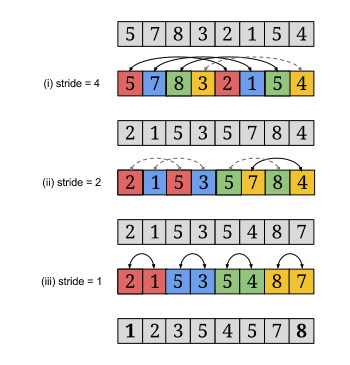
\includegraphics[width=0.5\textwidth]{images/minmax-example.png}
  \caption{Example run on an array of 8 values. 4 threads compare 2
    values at a time, swapping the values so that the smallest of them
  are to the left. At each step, the stride decreases. In the end, the
  smallest value is located at index 0, and the largest value is at
  index 7. The full arrows show values that need to be swapped, while
  the dotted shows values already in the correct place.}
  \label{minmax-example-figure}
\end{figure}


\subsection{Refinement kernels}


\subsubsection{Cross Checking}

As explained in section \ref{sect:cross-checking-theory},
cross-checking is function that compares the left and right disparity
maps, removing unreliable matches. Unreliable matches can occur from
occlusions, reflective surfaces, or a surface difficult for the used
aggregation window size to properly match.


The function is pretty straight forward:

\[ \mathlarger{| (D(x,y)_l - D(x - D(x,y)_l ,y)_r | > T} \]

At each coordinate, grab the left disparity value. The right disparity
value is then fetched at the same coordinates minus the left disparity
value. These two disparity values are compared, and if the absolute
difference is beneath some threshold (1-2 depth levels is a good
threshold), it is a good match and the left disparity value is written
to the left disparity map. If the absolute difference is greater, it's
an unreliable match and a 0 is written in that coordinate.

\begin{lstlisting}[label={lst:cross-check}, caption=Cross-checking
  function.]

  // Fist examine the left image

  int left = left_result[gid.y * WIDTH + gid.x];
  int right = right_result[gid.y * WIDTH + gid.x - left];

  if(abs(left - right) > THRESHOLD)
      new_left[gid.y * WIDTH + gid.x] = 0;
  else
      new_left[gid.y * WIDTH + gid.x] = left;


  // And the same for the right image

  left = left_result[gid.y * WIDTH + gid.x];
  right = right_result[gid.y * WIDTH + gid.x + right];

  if(abs(left - right) > THRESHOLD)
      new_right_result[gid.y * WIDTH + gid.x] = 0;
  else
      new_right_result[gid.y * WIDTH + gid.x] = right;

\end{lstlisting}

Figure \ref{fig:cross-check-results} shows the results with and
without cross-checking. The left column, especially along the left
side of depth discontinuities, contains a large spread of disparity
values. This is because the WTA strategy always selects a best match,
whether it is a correct match or not.

\begin{figure}

  \begin{subfigure}[b]{0.48\textwidth}
    \centering
    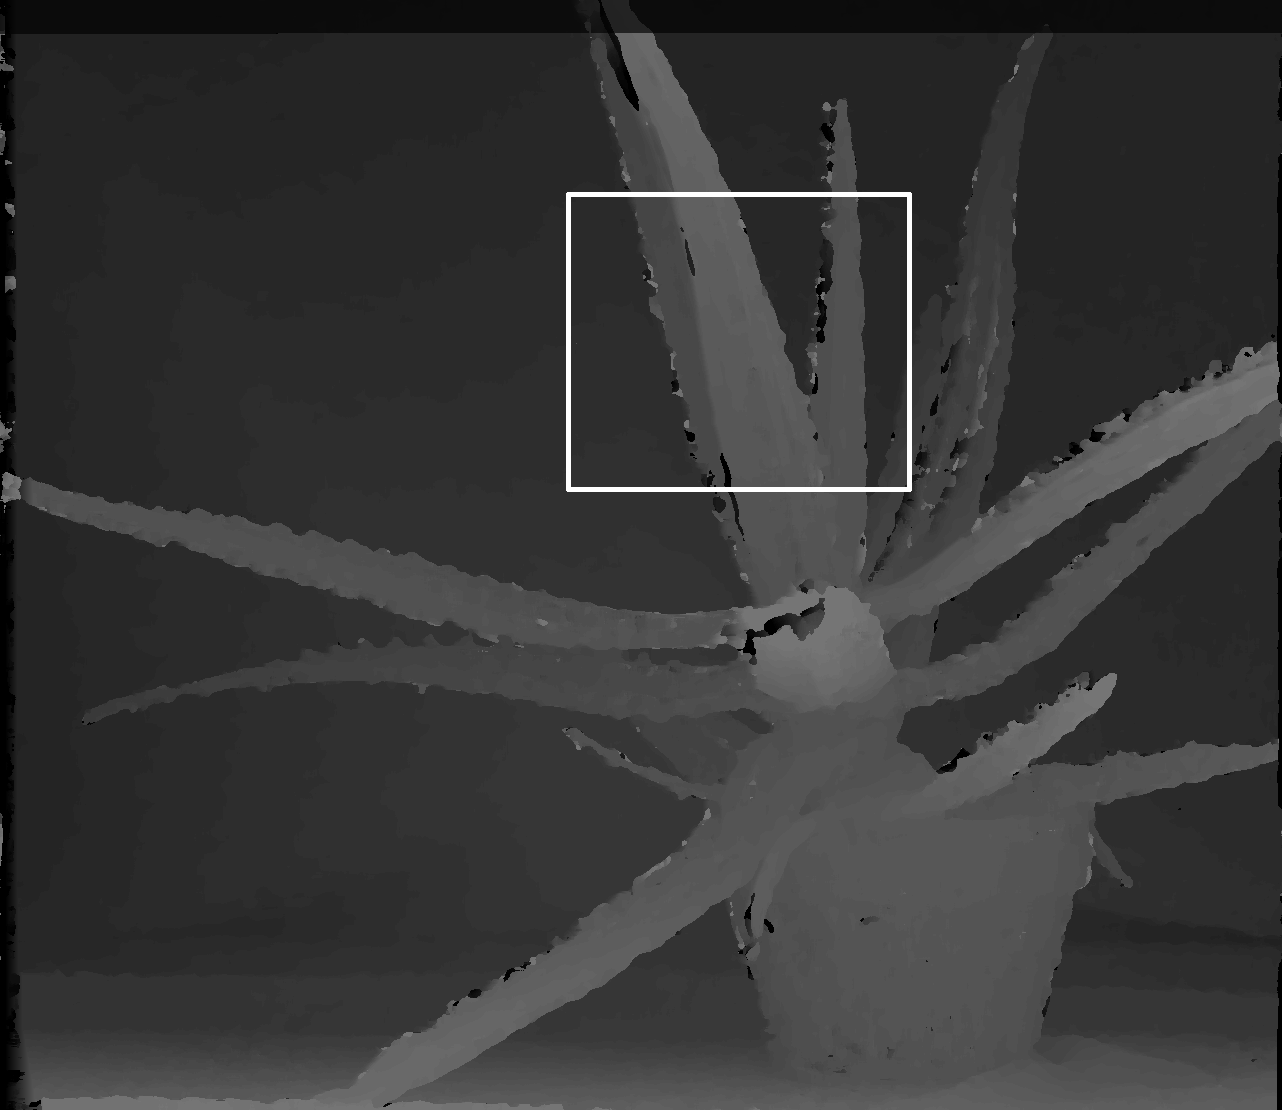
\includegraphics[width=\textwidth]{images/normal.png}
  \end{subfigure}
  ~
  \begin{subfigure}[b]{0.48\textwidth}
    \centering
    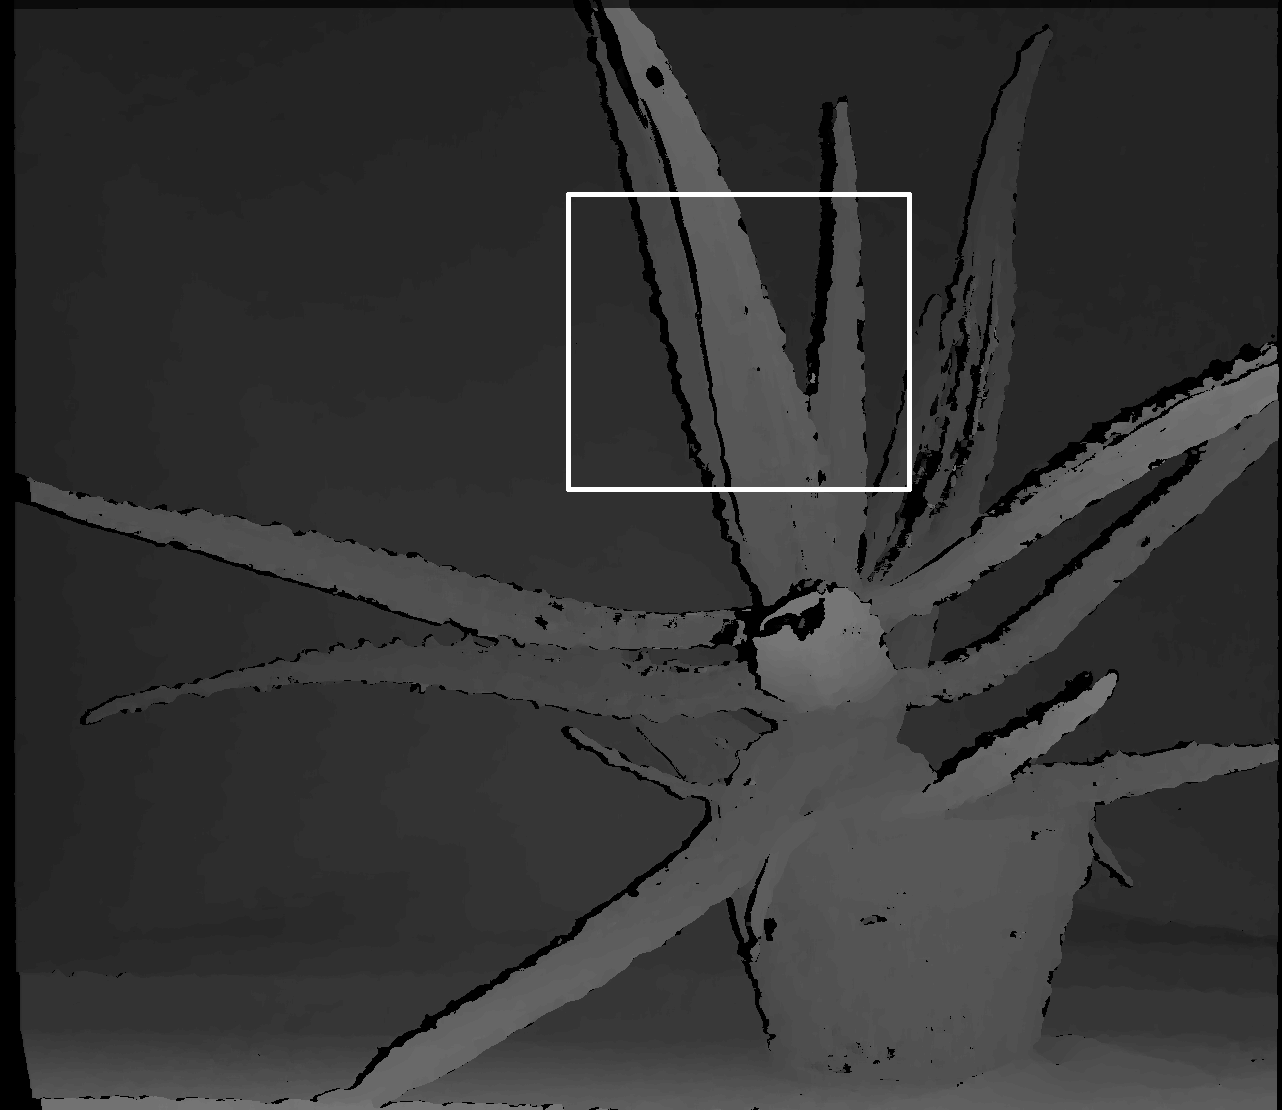
\includegraphics[width=\textwidth]{images/no-fill.png}
  \end{subfigure}

  \begin{subfigure}[b]{0.48\textwidth}
    \centering
    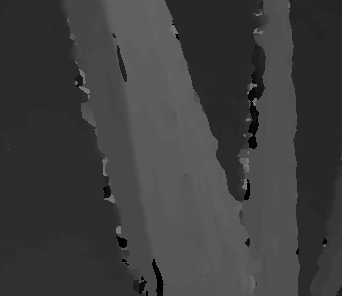
\includegraphics[width=\textwidth]{images/normal-zoomed.png}
    \caption{Without cross-checking}
  \end{subfigure}
  ~
  \begin{subfigure}[b]{0.48\textwidth}
    \centering
    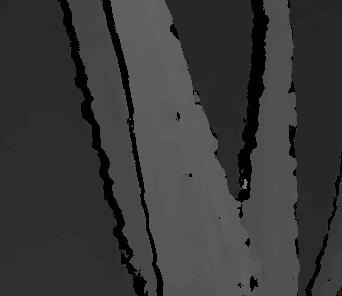
\includegraphics[width=\textwidth]{images/no-fill-zoomed.png}
    \caption{With cross-checking}
  \end{subfigure}

  \caption{Output without (column (a)) and with (column (b))
    cross-checking}

\end{figure}



\subsubsection{Occlusion Filling}

Scanline smearing. For every 

\begin{figure}

  \begin{subfigure}[b]{0.48\textwidth}
    \centering
    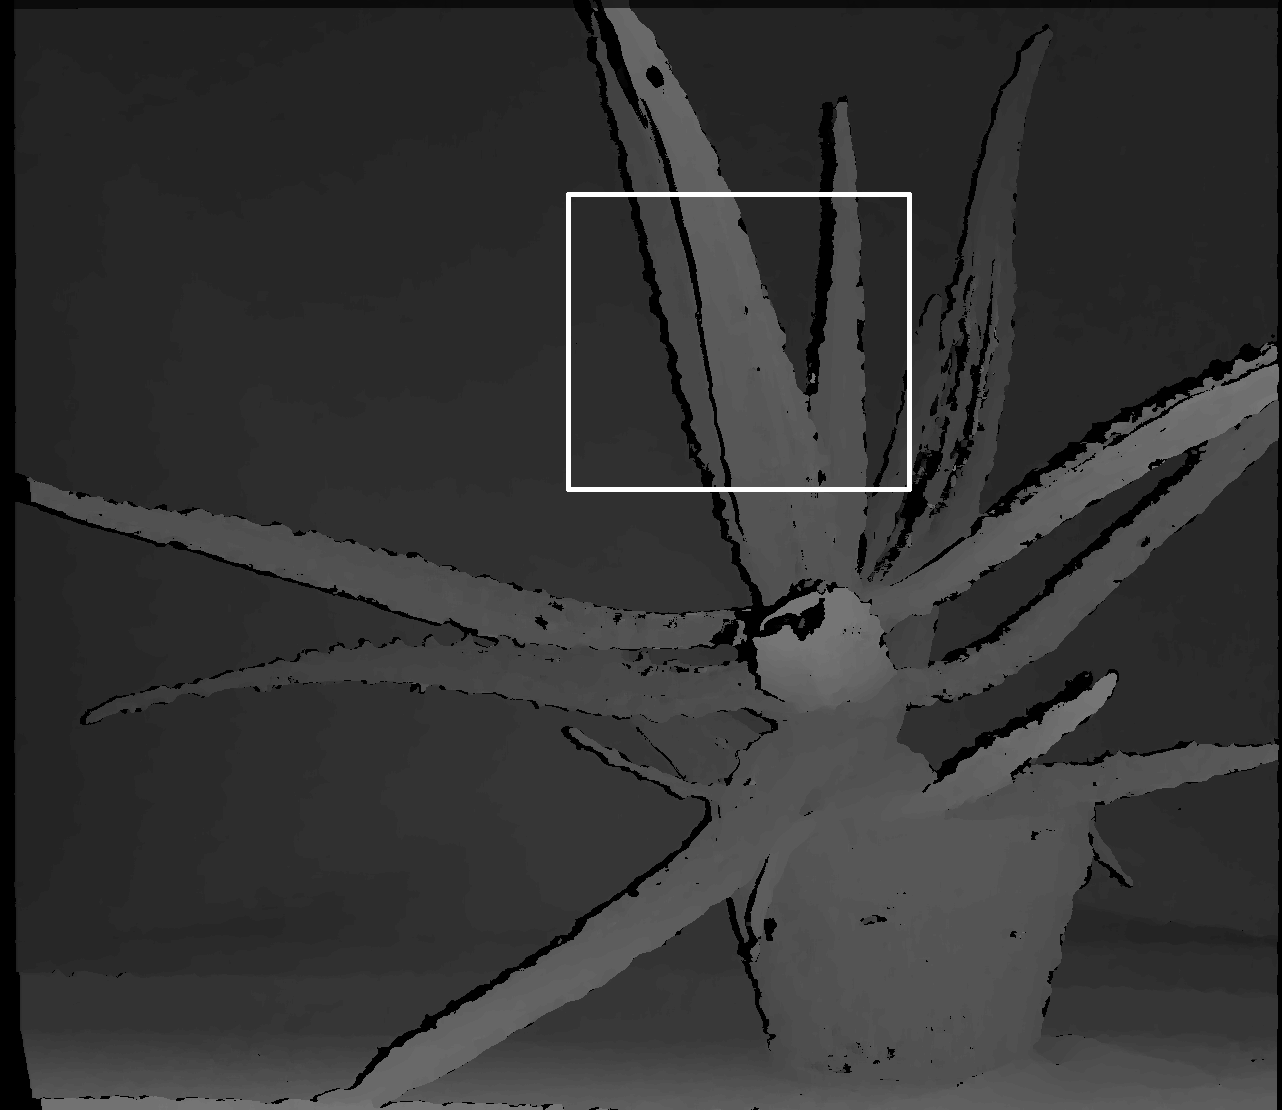
\includegraphics[width=\textwidth]{images/no-fill.png}
  \end{subfigure}
  ~
  \begin{subfigure}[b]{0.48\textwidth}
    \centering
    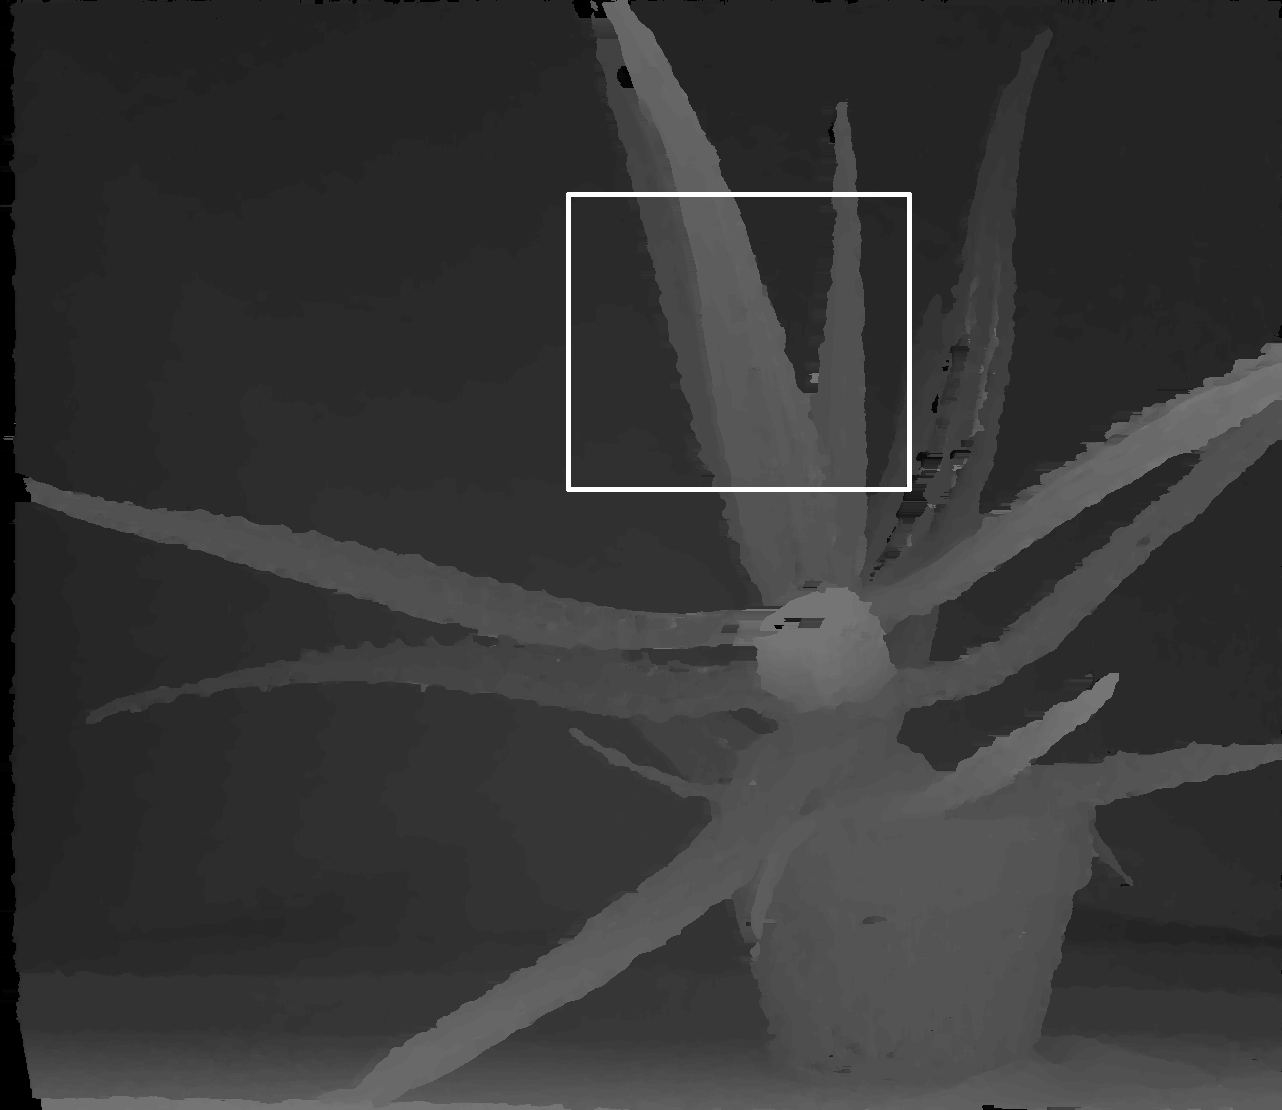
\includegraphics[width=\textwidth]{images/fill.png}
  \end{subfigure}

  \begin{subfigure}[b]{0.48\textwidth}
    \centering
    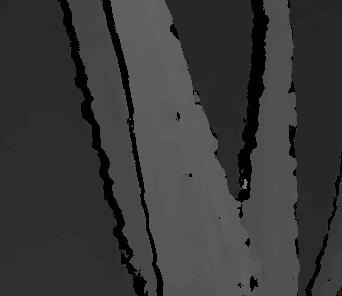
\includegraphics[width=\textwidth]{images/no-fill-zoomed.png}
    \caption{Unfilled occlusions}
  \end{subfigure}
  ~
  \begin{subfigure}[b]{0.48\textwidth}
    \centering
    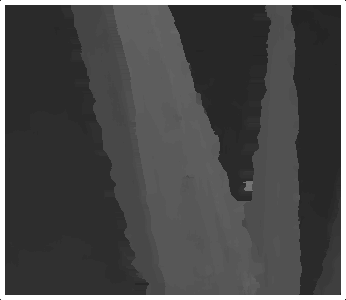
\includegraphics[width=\textwidth]{images/fill-zoomed.png}
    \caption{Filled occlusions}
  \end{subfigure}


\end{figure}



\subsubsection{Compute mask}
% Blockwise compute mask/map, workload management, creates

Sequential video frames contain a lot of redundant information,
especially when cameras remain fixed in position, always watching the
same scene.

Another way to reduce the number of computations is to avoid having to
calculate every disparity value for every frame. Sequential video
frames often have little variation. For example, the scene's
background is very likely to stay the same (unless the lighting
changes, or the camera is moved), so calculating these disparities is
a unnecessary.

One way to avoid re-calculating the same values for the next frame, is
by building a diff map. A binary image that indicates which pixels
have changed since the previous frame.

\chapter{Evaluation}

Performance measurements are done in two parts; the total run time of
the pipeline, and the output quality.

Run time is measured from the first input upload onto the device,
until the output is completely downloaded onto the host. Disparity map
quality is measured with Middlebury's excellent online disparity map
evaluator[TODO: reference Middlebury online evaluator].

The quality and run-time for the compute-map optimization is harder to
evaluate. The optimization only performs well on subsequent video
frames, and adds a small computation penalty to the start of each
frame. So testing it on a single set of images will not show the
performance benefits. A stereo rectified video sequence accompanied by
ground truth for each frame is needed, but well rectified and
relatively noise free video datasets don't yet exist.

Table \ref{algorithm-name-table} shows the name and properties of the
algorithms used when evaluating the run-time performance. Subsequent
algorithms include the previous algorithms properties, except for the
two DUAL algorithms, which were made with and without loop unrolling,
to demonstrate the huge difference it can make.

For quality, the BM algorithms are dropped, since they produce close
to identical results as DUAL, being essentially the same algorithm.
Some difference is found in erroneous areas, such as the input borders
(left side for the left inputs, right side for the right inputs) and
occlusion zones, due to some difference in the handling of the
aggregation window boundaries.

\begin{table}
  \begin{tabular}{|l|l|}
    \hline
    Algorithm name                     & Properties                                               \\
    \hline
    Block Matching (BM)                & No optimizations                                         \\
    Birchfield \& Tomasi (BT)          & BT cost matching method, instead of SAD. No optimizations\\
    Block Matching local memory (BMLM) & Local memory caching                                     \\
    Block Matching Unrolled (BMUR)     & Loop unrolling                                           \\
    Dual (DUAL)                        & Creates disparity map for both left and right input      \\
    Dual unrolled (DUALUR)             & Same as DUAL, but with loop unrolling                    \\
    Pyramid (PYRAMID)                  & Search range restriction                                 \\
    Pyramid minmax (MINMAX)            & Same as PYRAMID, but using the min-max function          \\
    \hline
  \end{tabular}
  \caption{Algorithm names and its properties. Each subsequent
    algorithm contains the previous' properties, except the DUALUR,
    which was included to demonstrate the power of loop unrolling.}
  \label{algorithm-name-table}
\end{table}


\subsection{Run time}

Figure [TODO: ref figure] shows a graph of the running times for the
different versions of the algorithm, with increasing maximum disparity
$\mathcal{D}$, along the X-axis.



\begin{figure}
  \centering
  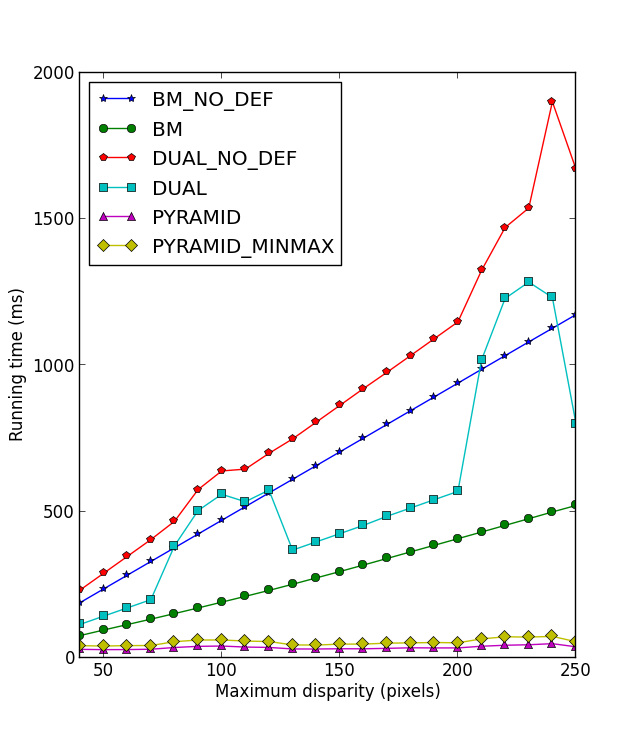
\includegraphics[width=0.8\textwidth]{images/runtime_9.png}
  \caption{Running time for each algorithm}
  \label{runtime-9}
\end{figure}


\subsection{Disparity map quality}

\begin{figure}
  \centering
  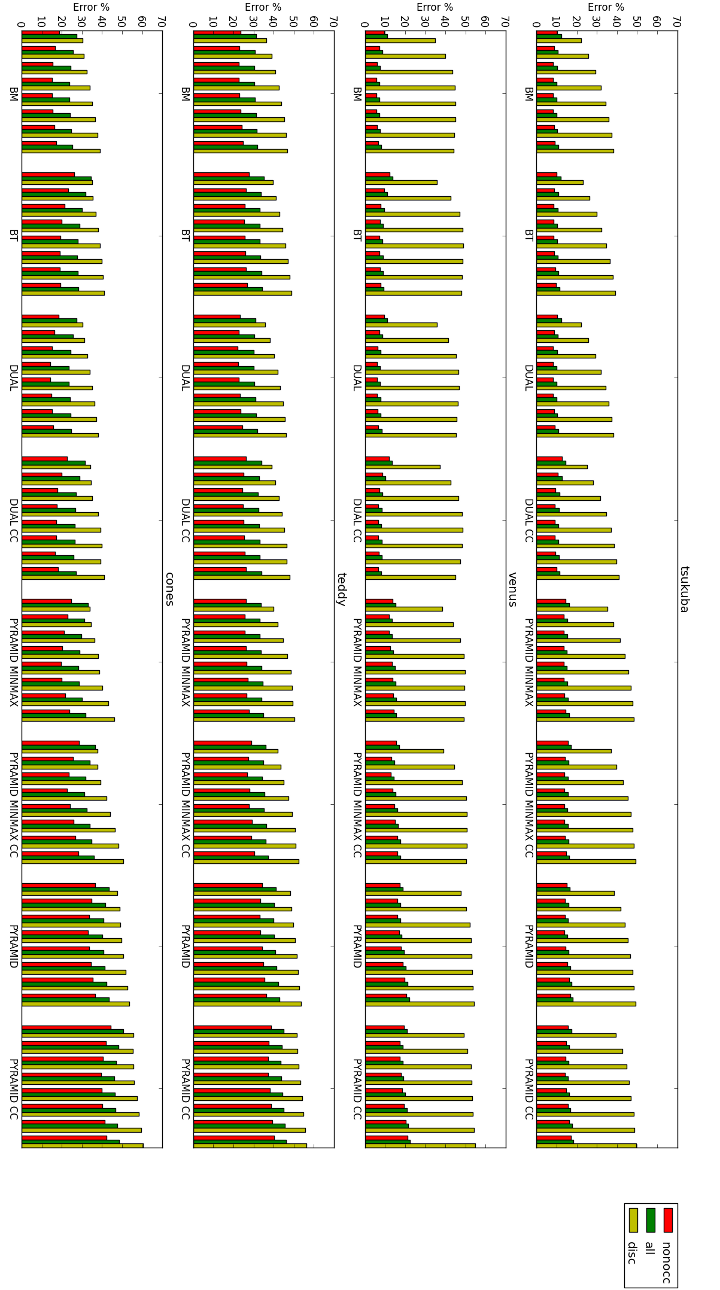
\includegraphics[width=\textwidth,height=\textheight]{images/quality_barchart_flipped.png}
  \caption{Error percentages for the datasets. Each graph contains
    groups of 3 * 8 bars, each representing increasing window sizes
    ranging from 7 up to 21 pixels}
  \label{quality-barchart}
\end{figure}


Figure \ref{quality-barchar} shows how the quality is affected by
increasing aggregation window size, $\omega$ $\times$ $\omega$. Each
of the four graphs are measurements on the four middlebury evaluation
datasets. In each graph, groups of 3 $\times$ 8 bars represent the
error percentages for non-occluded, all and discontinuity areas, with
increasing $\omega$ from 7 to 21. The algorithms used are labeled
beneath.

The notable features on the graph is the opposite trends of errors in
textureless areas and occlusions. In all instances, the increase of
$\omega$ results in a close to linear increase in errors in
occluded areas, while non-occluded areas are relatively constant, with
a few exceptions where the error rates decrease slightly.

Another noteworthy feature is that the algorithms using cross-checking
[TODO: ref cross-checking section] receives a higher error percentage
for occluded areas than the same algorithms without cross-checking.
This is because the evaluator also counts a disparity value of 0 as an
error, even in occluded areas. Non of the implemented algorithms
attempt to extrapolate disparities for occlusions, and therefor suffer
a higher error rate.

The algorithms not using cross-checking ends up with some disparity
value anywhere between 0 and max-disparity, which can be within the
threshold of what the evaluator considers an error. This can make the
cross-checking algorithms appear worse than its non-cross-checking
counterpart.

\begin{figure}
  \centering
  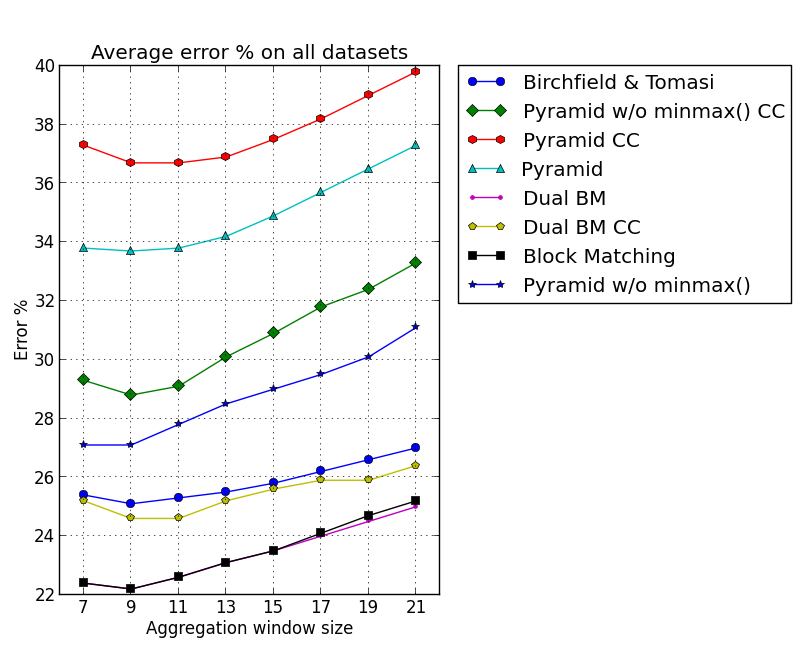
\includegraphics[width=\textwidth]{images/avg_error_all.png}
  \caption{Average error percentages for all the datasets. }
  \label{average-error-rates-final}
\end{figure}

The overall best quality is found by averaging error rates over all
four datasets, as shown in figure\ref{average-error-rates-final}. As
with most local algorithms, averaging the error rates is a trade-off
between the type of errors one considers most important.



\begin{figure}

  \setcounter{subfigure}{0}
  \label{fig:grid-of-outputs-tsukuba}
  \centering


  \begin{subfigure}[b]{0.45\textwidth}
    \centering
    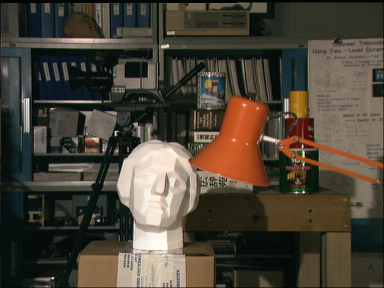
\includegraphics[width=\textwidth]{images/stereo-pairs/tsukuba_imL.png}
    \caption{Input}
  \end{subfigure}
  ~
  \begin{subfigure}[b]{0.45\textwidth}
    \centering
    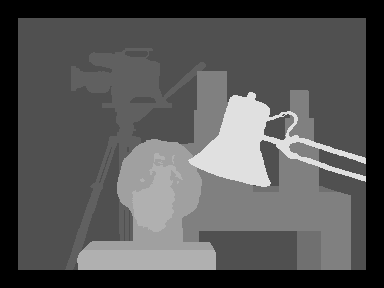
\includegraphics[width=\textwidth]{images/stereo-pairs/tsukuba_groundtruth.png}
    \caption{Ground truth}
  \end{subfigure}

  %
  %

  \begin{subfigure}[b]{0.23\textwidth}
    \centering
    
\includegraphics[width=\textwidth]{images/stereo-pairs/tsukuba_bm_9.png}
    \caption{BM 9}
  \end{subfigure}
  ~
  \begin{subfigure}[b]{0.23\textwidth}
    \centering
    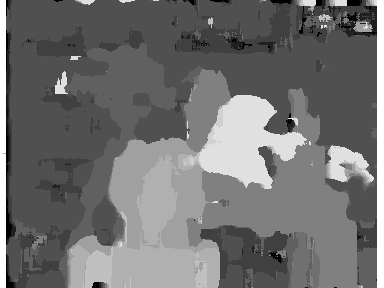
\includegraphics[width=\textwidth]{images/stereo-pairs/tsukuba_bm_13.png}
    \caption{BM 13}
  \end{subfigure}
  ~
  \begin{subfigure}[b]{0.23\textwidth}
    \centering
    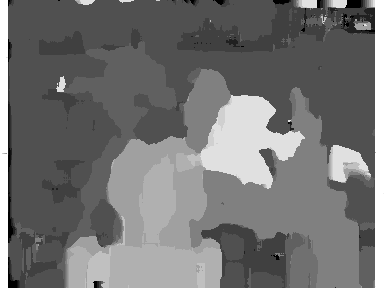
\includegraphics[width=\textwidth]{images/stereo-pairs/tsukuba_bm_17.png}
    \caption{BM 17}
  \end{subfigure}
  ~
  \begin{subfigure}[b]{0.23\textwidth}
    \centering
    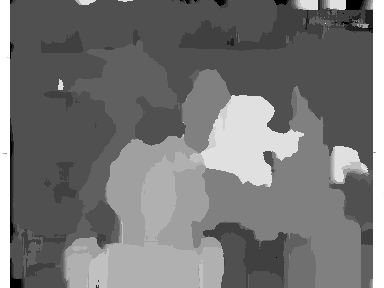
\includegraphics[width=\textwidth]{images/stereo-pairs/tsukuba_bm_21.png}
    \caption{BM 21}
  \end{subfigure}

  %
  %

  \begin{subfigure}[b]{0.23\textwidth}
    \centering
    
\includegraphics[width=\textwidth]{images/stereo-pairs/tsukuba_bt_9.png}
    \caption{BT 9}
  \end{subfigure}
  ~
  \begin{subfigure}[b]{0.23\textwidth}
    \centering
    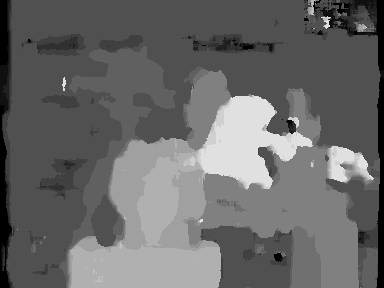
\includegraphics[width=\textwidth]{images/stereo-pairs/tsukuba_bt_13.png}
    \caption{BT 13}
  \end{subfigure}
  ~
  \begin{subfigure}[b]{0.23\textwidth}
    \centering
    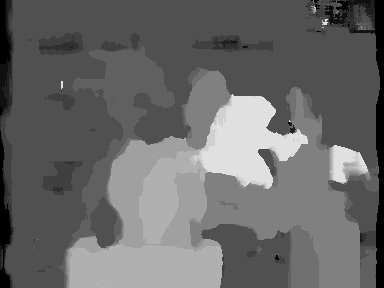
\includegraphics[width=\textwidth]{images/stereo-pairs/tsukuba_bt_17.png}
    \caption{BT 17}
  \end{subfigure}
  ~
  \begin{subfigure}[b]{0.23\textwidth}
    \centering
    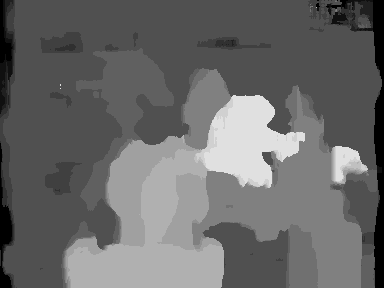
\includegraphics[width=\textwidth]{images/stereo-pairs/tsukuba_bt_21.png}
    \caption{BT 21}
  \end{subfigure}

  %
  %

  \begin{subfigure}[b]{0.23\textwidth}
    \centering
    
\includegraphics[width=\textwidth]{images/stereo-pairs/tsukuba_dual_crosschecked_9.png}
    \caption{CC 9}
  \end{subfigure}
  ~
  \begin{subfigure}[b]{0.23\textwidth}
    \centering
    
\includegraphics[width=\textwidth]{images/stereo-pairs/tsukuba_dual_crosschecked_13.png}
    \caption{CC 13}
  \end{subfigure}
  ~
  \begin{subfigure}[b]{0.23\textwidth}
    \centering
    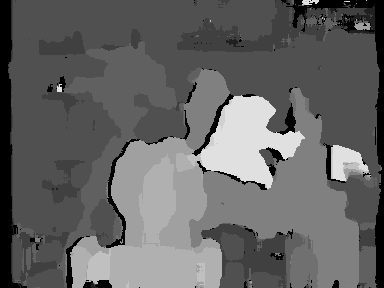
\includegraphics[width=\textwidth]{images/stereo-pairs/tsukuba_dual_crosschecked_17.png}
    \caption{CC 17}
  \end{subfigure}
  ~
  \begin{subfigure}[b]{0.23\textwidth}
    \centering
    
\includegraphics[width=\textwidth]{images/stereo-pairs/tsukuba_dual_crosschecked_21.png}
    \caption{CC 21}
  \end{subfigure}

  %
  %

  \begin{subfigure}[b]{0.23\textwidth}
    \centering
    
\includegraphics[width=\textwidth]{images/stereo-pairs/tsukuba_pyramid_9.png}
    \caption{PY 9}
  \end{subfigure}
  ~
  \begin{subfigure}[b]{0.23\textwidth}
    \centering
    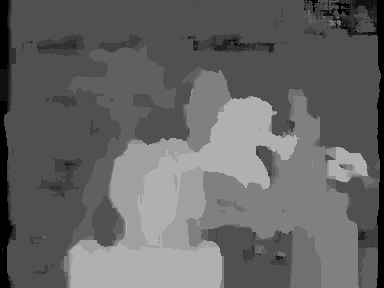
\includegraphics[width=\textwidth]{images/stereo-pairs/tsukuba_pyramid_13.png}
    \caption{PY 13}
  \end{subfigure}
  ~
  \begin{subfigure}[b]{0.23\textwidth}
    \centering
    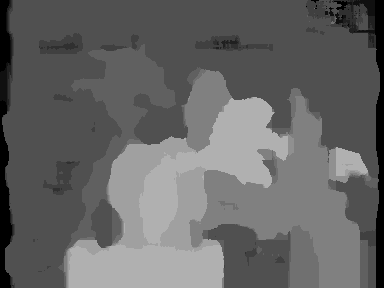
\includegraphics[width=\textwidth]{images/stereo-pairs/tsukuba_pyramid_17.png}
    \caption{PY 17}
  \end{subfigure}
  ~
  \begin{subfigure}[b]{0.23\textwidth}
    \centering
    \includegraphics[width=\textwidth]{images/stereo-pairs/tsukuba_pyramid_21.png}
    \caption{PY 21}
  \end{subfigure}

  %
  %

  \begin{subfigure}[b]{0.23\textwidth}
    \centering
    \includegraphics[width=\textwidth]{images/stereo-pairs/tsukuba_pyramid_crosschecked_9.png}
    \caption{PY CC 9}
  \end{subfigure}
  ~
  \begin{subfigure}[b]{0.23\textwidth}
    \centering
    \includegraphics[width=\textwidth]{images/stereo-pairs/tsukuba_pyramid_crosschecked_13.png}
    \caption{PY CC 13}
  \end{subfigure}
  ~
  \begin{subfigure}[b]{0.23\textwidth}
    \centering
    \includegraphics[width=\textwidth]{images/stereo-pairs/tsukuba_pyramid_crosschecked_17.png}
    \caption{PY CC 17}
  \end{subfigure}
  ~
  \begin{subfigure}[b]{0.23\textwidth}
    \centering
    \includegraphics[width=\textwidth]{images/stereo-pairs/tsukuba_pyramid_crosschecked_21.png}
    \caption{PY CC 21}
  \end{subfigure}

  \caption{Tsukuba dataset}

\end{figure}



\begin{figure}
  \setcounter{subfigure}{0}
  \label{fig:grid-of-outputs-venus}
  \centering



  \begin{subfigure}[b]{0.3\textwidth}
    \centering
    \includegraphics[width=\textwidth]{images/stereo-pairs/venus_imL.png}
    \caption{Input}
  \end{subfigure}
  ~
  \begin{subfigure}[b]{0.3\textwidth}
    \centering
    \includegraphics[width=\textwidth]{images/stereo-pairs/venus_groundtruth.png}
    \caption{Ground truth}
  \end{subfigure}

  %
  %

  \begin{subfigure}[b]{0.23\textwidth}
    \centering
    \includegraphics[width=\textwidth]{images/stereo-pairs/venus_bm_9.png}
    \caption{BM 9}
  \end{subfigure}
  ~
  \begin{subfigure}[b]{0.23\textwidth}
    \centering
    \includegraphics[width=\textwidth]{images/stereo-pairs/venus_bm_13.png}
    \caption{BM 13}
  \end{subfigure}
  ~
  \begin{subfigure}[b]{0.23\textwidth}
    \centering
    \includegraphics[width=\textwidth]{images/stereo-pairs/venus_bm_17.png}
    \caption{BM 17}
  \end{subfigure}
  ~
  \begin{subfigure}[b]{0.23\textwidth}
    \centering
    \includegraphics[width=\textwidth]{images/stereo-pairs/venus_bm_21.png}
    \caption{BM 21}
  \end{subfigure}

  %
  %

  \begin{subfigure}[b]{0.23\textwidth}
    \centering
    \includegraphics[width=\textwidth]{images/stereo-pairs/venus_bt_9.png}
    \caption{BT 9}
  \end{subfigure}
  ~
  \begin{subfigure}[b]{0.23\textwidth}
    \centering
    \includegraphics[width=\textwidth]{images/stereo-pairs/venus_bt_13.png}
    \caption{BT 13}
  \end{subfigure}
  ~
  \begin{subfigure}[b]{0.23\textwidth}
    \centering
    \includegraphics[width=\textwidth]{images/stereo-pairs/venus_bt_17.png}
    \caption{BT 17}
  \end{subfigure}
  ~
  \begin{subfigure}[b]{0.23\textwidth}
    \centering
    \includegraphics[width=\textwidth]{images/stereo-pairs/venus_bt_21.png}
    \caption{BT 21}
  \end{subfigure}

  %
  %

  \begin{subfigure}[b]{0.23\textwidth}
    \centering
    \includegraphics[width=\textwidth]{images/stereo-pairs/venus_dual_crosschecked_9.png}
    \caption{CC 9}
  \end{subfigure}
  ~
  \begin{subfigure}[b]{0.23\textwidth}
    \centering
    \includegraphics[width=\textwidth]{images/stereo-pairs/venus_dual_crosschecked_13.png}
    \caption{CC 13}
  \end{subfigure}
  ~
  \begin{subfigure}[b]{0.23\textwidth}
    \centering
    \includegraphics[width=\textwidth]{images/stereo-pairs/venus_dual_crosschecked_17.png}
    \caption{CC 17}
  \end{subfigure}
  ~
  \begin{subfigure}[b]{0.23\textwidth}
    \centering
    \includegraphics[width=\textwidth]{images/stereo-pairs/venus_dual_crosschecked_21.png}
    \caption{CC 21}
  \end{subfigure}

  %
  %

  \begin{subfigure}[b]{0.23\textwidth}
    \centering
    \includegraphics[width=\textwidth]{images/stereo-pairs/venus_pyramid_9.png}
    \caption{PY 9}
  \end{subfigure}
  ~
  \begin{subfigure}[b]{0.23\textwidth}
    \centering
    \includegraphics[width=\textwidth]{images/stereo-pairs/venus_pyramid_13.png}
    \caption{PY 13}
  \end{subfigure}
  ~
  \begin{subfigure}[b]{0.23\textwidth}
    \centering
    \includegraphics[width=\textwidth]{images/stereo-pairs/venus_pyramid_17.png}
    \caption{PY 17}
  \end{subfigure}
  ~
  \begin{subfigure}[b]{0.23\textwidth}
    \centering
    \includegraphics[width=\textwidth]{images/stereo-pairs/venus_pyramid_21.png}
    \caption{PY 21}
  \end{subfigure}

  %
  %

  \begin{subfigure}[b]{0.23\textwidth}
    \centering
    \includegraphics[width=\textwidth]{images/stereo-pairs/venus_pyramid_crosschecked_9.png}
    \caption{PY CC 9}
  \end{subfigure}
  ~
  \begin{subfigure}[b]{0.23\textwidth}
    \centering
    \includegraphics[width=\textwidth]{images/stereo-pairs/venus_pyramid_crosschecked_13.png}
    \caption{PY CC 13}
  \end{subfigure}
  ~
  \begin{subfigure}[b]{0.23\textwidth}
    \centering
    \includegraphics[width=\textwidth]{images/stereo-pairs/venus_pyramid_crosschecked_17.png}
    \caption{PY CC 17}
  \end{subfigure}
  ~
  \begin{subfigure}[b]{0.23\textwidth}
    \centering
    \includegraphics[width=\textwidth]{images/stereo-pairs/venus_pyramid_crosschecked_21.png}
    \caption{PY CC 21}
  \end{subfigure}

  \caption{Venus dataset}

\end{figure}

\begin{figure}
  \setcounter{subfigure}{0}

  \label{fig:grid-of-outputs-teddy}
  \centering


  \begin{subfigure}[b]{0.45\textwidth}
    \centering
    \includegraphics[width=\textwidth]{images/stereo-pairs/teddy_imL.png}
    \caption{Input}
  \end{subfigure}
  ~
  \begin{subfigure}[b]{0.45\textwidth}
    \centering
    \includegraphics[width=\textwidth]{images/stereo-pairs/teddy_groundtruth.png}
    \caption{Ground truth}
  \end{subfigure}

  %
  %

  \begin{subfigure}[b]{0.23\textwidth}
    \centering
    \includegraphics[width=\textwidth]{images/stereo-pairs/teddy_bm_9.png}
    \caption{BM 9}
  \end{subfigure}
  ~
  \begin{subfigure}[b]{0.23\textwidth}
    \centering
    \includegraphics[width=\textwidth]{images/stereo-pairs/teddy_bm_13.png}
    \caption{BM 13}
  \end{subfigure}
  ~
  \begin{subfigure}[b]{0.23\textwidth}
    \centering
    \includegraphics[width=\textwidth]{images/stereo-pairs/teddy_bm_17.png}
    \caption{BM 17}
  \end{subfigure}
  ~
  \begin{subfigure}[b]{0.23\textwidth}
    \centering
    \includegraphics[width=\textwidth]{images/stereo-pairs/teddy_bm_21.png}
    \caption{BM 21}
  \end{subfigure}




  \begin{subfigure}[b]{0.23\textwidth}
    \centering
    \includegraphics[width=\textwidth]{images/stereo-pairs/teddy_bt_9.png}
    \caption{BT 9}
  \end{subfigure}
  ~
  \begin{subfigure}[b]{0.23\textwidth}
    \centering
    \includegraphics[width=\textwidth]{images/stereo-pairs/teddy_bt_13.png}
    \caption{BT 13}
  \end{subfigure}
  ~
  \begin{subfigure}[b]{0.23\textwidth}
    \centering
    \includegraphics[width=\textwidth]{images/stereo-pairs/teddy_bt_17.png}
    \caption{BT 17}
  \end{subfigure}
  ~
  \begin{subfigure}[b]{0.23\textwidth}
    \centering
    \includegraphics[width=\textwidth]{images/stereo-pairs/teddy_bt_21.png}
    \caption{BT 21}
  \end{subfigure}




  \begin{subfigure}[b]{0.23\textwidth}
    \centering
    \includegraphics[width=\textwidth]{images/stereo-pairs/teddy_dual_crosschecked_9.png}
    \caption{CC 9}
  \end{subfigure}
  ~
  \begin{subfigure}[b]{0.23\textwidth}
    \centering
    \includegraphics[width=\textwidth]{images/stereo-pairs/teddy_dual_crosschecked_13.png}
    \caption{CC 13}
  \end{subfigure}
  ~
  \begin{subfigure}[b]{0.23\textwidth}
    \centering
    \includegraphics[width=\textwidth]{images/stereo-pairs/teddy_dual_crosschecked_17.png}
    \caption{CC 17}
  \end{subfigure}
  ~
  \begin{subfigure}[b]{0.23\textwidth}
    \centering
    \includegraphics[width=\textwidth]{images/stereo-pairs/teddy_dual_crosschecked_21.png}
    \caption{CC 21}
  \end{subfigure}




  \begin{subfigure}[b]{0.23\textwidth}
    \centering
    \includegraphics[width=\textwidth]{images/stereo-pairs/teddy_pyramid_9.png}
    \caption{PY 9}
  \end{subfigure}
  ~
  \begin{subfigure}[b]{0.23\textwidth}
    \centering
    \includegraphics[width=\textwidth]{images/stereo-pairs/teddy_pyramid_13.png}
    \caption{PY 13}
  \end{subfigure}
  ~
  \begin{subfigure}[b]{0.23\textwidth}
    \centering
    \includegraphics[width=\textwidth]{images/stereo-pairs/teddy_pyramid_17.png}
    \caption{PY 17}
  \end{subfigure}
  ~
  \begin{subfigure}[b]{0.23\textwidth}
    \centering
    \includegraphics[width=\textwidth]{images/stereo-pairs/teddy_pyramid_21.png}
    \caption{PY 21}
  \end{subfigure}




  \begin{subfigure}[b]{0.23\textwidth}
    \centering
    \includegraphics[width=\textwidth]{images/stereo-pairs/teddy_pyramid_crosschecked_9.png}
    \caption{PY CC 9}
  \end{subfigure}
  ~
  \begin{subfigure}[b]{0.23\textwidth}
    \centering
    \includegraphics[width=\textwidth]{images/stereo-pairs/teddy_pyramid_crosschecked_13.png}
    \caption{PY CC 13}
  \end{subfigure}
  ~
  \begin{subfigure}[b]{0.23\textwidth}
    \centering
    \includegraphics[width=\textwidth]{images/stereo-pairs/teddy_pyramid_crosschecked_17.png}
    \caption{PY CC 17}
  \end{subfigure}
  ~
  \begin{subfigure}[b]{0.23\textwidth}
    \centering
    \includegraphics[width=\textwidth]{images/stereo-pairs/teddy_pyramid_crosschecked_21.png}
    \caption{PY CC 21}
  \end{subfigure}

  \caption{Teddy dataset}

\end{figure}


\begin{figure}
  \setcounter{subfigure}{0}

  \label{fig:grid-of-outputs-cones}
  \centering


  \begin{subfigure}[b]{0.45\textwidth}
    \centering
    \includegraphics[width=\textwidth]{images/stereo-pairs/cones_imL.png}
    \caption{Input}
  \end{subfigure}
  ~
  \begin{subfigure}[b]{0.45\textwidth}
    \centering
    \includegraphics[width=\textwidth]{images/stereo-pairs/cones_groundtruth.png}
    \caption{Ground truth}
  \end{subfigure}

  %
  %

  \begin{subfigure}[b]{0.23\textwidth}
    \centering
    \includegraphics[width=\textwidth]{images/stereo-pairs/cones_bm_9.png}
    \caption{BM 9}
  \end{subfigure}
  ~
  \begin{subfigure}[b]{0.23\textwidth}
    \centering
    \includegraphics[width=\textwidth]{images/stereo-pairs/cones_bm_13.png}
    \caption{BM 13}
  \end{subfigure}
  ~
  \begin{subfigure}[b]{0.23\textwidth}
    \centering
    \includegraphics[width=\textwidth]{images/stereo-pairs/cones_bm_17.png}
    \caption{BM 17}
  \end{subfigure}
  ~
  \begin{subfigure}[b]{0.23\textwidth}
    \centering
    \includegraphics[width=\textwidth]{images/stereo-pairs/cones_bm_21.png}
    \caption{BM 21}
  \end{subfigure}

  %
  %

  \begin{subfigure}[b]{0.23\textwidth}
    \centering
    \includegraphics[width=\textwidth]{images/stereo-pairs/cones_bt_9.png}
    \caption{BT 9}
  \end{subfigure}
  ~
  \begin{subfigure}[b]{0.23\textwidth}
    \centering
    \includegraphics[width=\textwidth]{images/stereo-pairs/cones_bt_13.png}
    \caption{BT 13}
  \end{subfigure}
  ~
  \begin{subfigure}[b]{0.23\textwidth}
    \centering
    \includegraphics[width=\textwidth]{images/stereo-pairs/cones_bt_17.png}
    \caption{BT 17}
  \end{subfigure}
  ~
  \begin{subfigure}[b]{0.23\textwidth}
    \centering
    \includegraphics[width=\textwidth]{images/stereo-pairs/cones_bt_21.png}
    \caption{BT 21}
  \end{subfigure}

  %
  %

  \begin{subfigure}[b]{0.23\textwidth}
    \centering
    \includegraphics[width=\textwidth]{images/stereo-pairs/cones_dual_crosschecked_9.png}
    \caption{CC 9}
  \end{subfigure}
  ~
  \begin{subfigure}[b]{0.23\textwidth}
    \centering
    \includegraphics[width=\textwidth]{images/stereo-pairs/cones_dual_crosschecked_13.png}
    \caption{CC 13}
  \end{subfigure}
  ~
  \begin{subfigure}[b]{0.23\textwidth}
    \centering
    \includegraphics[width=\textwidth]{images/stereo-pairs/cones_dual_crosschecked_17.png}
    \caption{CC 17}
  \end{subfigure}
  ~
  \begin{subfigure}[b]{0.23\textwidth}
    \centering
    \includegraphics[width=\textwidth]{images/stereo-pairs/cones_dual_crosschecked_21.png}
    \caption{CC 21}
  \end{subfigure}

  %
  %

  \begin{subfigure}[b]{0.23\textwidth}
    \centering
    \includegraphics[width=\textwidth]{images/stereo-pairs/cones_pyramid_9.png}
    \caption{PY 9}
  \end{subfigure}
  ~
  \begin{subfigure}[b]{0.23\textwidth}
    \centering
    \includegraphics[width=\textwidth]{images/stereo-pairs/cones_pyramid_13.png}
    \caption{PY 13}
  \end{subfigure}
  ~
  \begin{subfigure}[b]{0.23\textwidth}
    \centering
    \includegraphics[width=\textwidth]{images/stereo-pairs/cones_pyramid_17.png}
    \caption{PY 17}
  \end{subfigure}
  ~
  \begin{subfigure}[b]{0.23\textwidth}
    \centering
    \includegraphics[width=\textwidth]{images/stereo-pairs/cones_pyramid_21.png}
    \caption{PY 21}
  \end{subfigure}

  %
  %

  \begin{subfigure}[b]{0.23\textwidth}
    \centering
    \includegraphics[width=\textwidth]{images/stereo-pairs/cones_pyramid_crosschecked_9.png}
    \caption{PY CC 9}
  \end{subfigure}
  ~
  \begin{subfigure}[b]{0.23\textwidth}
    \centering
    \includegraphics[width=\textwidth]{images/stereo-pairs/cones_pyramid_crosschecked_13.png}
    \caption{PY CC 13}
  \end{subfigure}
  ~
  \begin{subfigure}[b]{0.23\textwidth}
    \centering
    \includegraphics[width=\textwidth]{images/stereo-pairs/cones_pyramid_crosschecked_17.png}
    \caption{PY CC 17}
  \end{subfigure}
  ~
  \begin{subfigure}[b]{0.23\textwidth}
    \centering
    \includegraphics[width=\textwidth]{images/stereo-pairs/cones_pyramid_crosschecked_21.png}
    \caption{PY CC 21}
  \end{subfigure}

  \caption{Cones dataset}

\end{figure}

\begin{table}
    \begin{tabular}{|l|l|l|l|l|l|l|}
        \hline
        disparity & BM\_NO\_DEF & BM     & DUAL\_NO\_DEF & DUAL    & PYRAMID & MINMAX \\ \hline
        50 & 188.70    & 76.18  & 231.81      & 114.36  & 29.14   & 41.77          \\
        60 & 235.67    & 95.22  & 289.25      & 142.68  & 28.18   & 40.44          \\
        70 & 282.57    & 113.80 & 346.73      & 170.83  & 28.35   & 41.95          \\
        80 & 329.52    & 132.39 & 404.38      & 199.02  & 29.55   & 42.25          \\
        90 & 376.42    & 151.40 & 466.80      & 383.05  & 35.47   & 55.27          \\
        100 & 423.41    & 170.64 & 575.43      & 503.63  & 39.40   & 61.07          \\
       110 & 470.31    & 190.44 & 639.04      & 559.31  & 40.48   & 61.24          \\
        120 & 517.05    & 210.34 & 645.30      & 533.80  & 37.00   & 57.42          \\
        130 & 563.85    & 230.64 & 699.17      & 573.71  & 35.74   & 55.89          \\
        140 & 610.49    & 251.62 & 748.59      & 368.40  & 30.46   & 44.37          \\
        150 & 657.21    & 273.35 & 805.79      & 396.54  & 30.31   & 43.71          \\
        160 & 704.13    & 295.04 & 863.08      & 424.75  & 31.18   & 47.09          \\
        170 & 751.17    & 317.43 & 920.68      & 453.04  & 31.02   & 47.12          \\
        180 & 798.22    & 339.84 & 976.49      & 484.16  & 32.58   & 50.35          \\
        190 & 845.26    & 362.44 & 1033.66     & 512.42  & 34.46   & 51.28          \\
        200 & 892.14    & 384.89 & 1091.29     & 540.90  & 33.98   & 52.54          \\
        210 & 939.28    & 407.46 & 1148.60     & 569.16  & 34.04   & 51.51          \\
        220 & 986.41    & 430.19 & 1324.52     & 1018.30 & 39.81   & 64.96          \\
        230 & 1033.23   & 453.00 & 1471.33     & 1229.00 & 43.17   & 72.08          \\
        240 & 1080.22   & 475.77 & 1538.02     & 1284.77 & 44.88   & 71.05          \\
        250 & 1126.74   & 498.85 & 1901.21     & 1232.11 & 48.57   & 73.48          \\
        \hline
    \end{tabular}
    \caption{Run times in milliseconds for each algorithm run at
      increasing search ranges}
\end{table}

\begin{tabular}{|l|l|l||l|l|l||l|l|l||l|l|l||l|}
  \hline
  \multicolumn{3}{|c||}{Tsukuba} &
  \multicolumn{3}{c||}{Venus} &
  \multicolumn{3}{c||}{Teddy} &
  \multicolumn{3}{c||}{Cones} & ~ \\
  \hline
  nocc & all & disc & nocc & all & disc & nocc & all & disc & nocc & all & disc & avg err\\
  \hline
  \multicolumn{13}{|c|}{Normal Block Matching} \\
  \hline
  10.4 & 12.3 & 22.3 & 9.62 & 11.1 & 35.0 & 23.6 & 31.3 & 36.4 & 18.8 & 27.5 & 30.2 & 22.4 \\
  8.79 & 10.7 & 25.7 & 7.14 & 8.67 & 40.1 & 22.9 & 30.6 & 38.9 & 16.7 & 25.6 & 30.9 & 22.2 \\
  8.24 & 10.2 & 29.4 & 6.17 & 7.69 & 43.6 & 22.6 & 30.3 & 40.7 & 15.6 & 24.4 & 32.4 & 22.6 \\
  8.09 & 9.91 & 32.1 & 5.79 & 7.30 & 44.9 & 22.8 & 30.5 & 42.6 & 15.1 & 23.9 & 33.9 & 23.1 \\
  8.14 & 9.88 & 34.3 & 5.70 & 7.19 & 45.2 & 23.1 & 30.8 & 43.9 & 15.1 & 23.8 & 35.1 & 23.5 \\
  8.33 & 10.0 & 36.0 & 5.84 & 7.30 & 45.0 & 23.6 & 31.2 & 45.3 & 15.6 & 24.2 & 36.5 & 24.1 \\
  8.76 & 10.4 & 37.4 & 6.10 & 7.54 & 44.6 & 24.1 & 31.6 & 46.2 & 16.4 & 24.8 & 37.9 & 24.7 \\
  9.24 & 10.9 & 38.4 & 6.61 & 8.02 & 44.1 & 24.7 & 32.0 & 46.8 & 17.1 & 25.3 & 38.9 & 25.2 \\
  \hline
  \multicolumn{13}{|c|}{Block Matching with Birchfield \& Tomasi matching} \\
  \hline
  10.1 & 12.0 & 23.0 & 12.4 & 13.9 & 35.8 & 27.6 & 35.1 & 39.7 & 26.2 & 34.4 & 35.0 & 25.4 \\
  8.92 & 10.9 & 26.4 & 9.54 & 11.1 & 42.8 & 26.2 & 33.7 & 41.2 & 23.2 & 31.7 & 35.4 & 25.1 \\
  8.58 & 10.6 & 29.8 & 7.95 & 9.52 & 47.2 & 25.6 & 33.2 & 43.0 & 21.5 & 30.1 & 36.8 & 25.3 \\
  8.51 & 10.4 & 32.4 & 7.43 & 9.00 & 48.6 & 25.4 & 33.0 & 44.4 & 20.0 & 28.8 & 38.0 & 25.5 \\
  8.61 & 10.4 & 34.6 & 7.28 & 8.84 & 48.9 & 25.5 & 33.1 & 45.8 & 19.2 & 28.0 & 39.0 & 25.8 \\
  8.83 & 10.6 & 36.4 & 7.34 & 8.91 & 48.7 & 25.9 & 33.5 & 47.2 & 19.0 & 27.8 & 39.9 & 26.2 \\
  9.26 & 11.0 & 38.0 & 7.50 & 9.09 & 48.3 & 26.3 & 33.9 & 48.1 & 19.1 & 27.9 & 40.5 & 26.6 \\
  9.67 & 11.4 & 39.2 & 7.74 & 9.33 & 48.0 & 26.9 & 34.4 & 48.8 & 19.4 & 28.2 & 41.2 & 27.0 \\
  \hline
  \multicolumn{13}{|c|}{Block Matching with left \& right disparity map} \\
  \hline
  10.4 & 12.3 & 22.3 & 9.71 & 11.2 & 35.9 & 23.4 & 31.1 & 35.9 & 18.5 & 27.4 & 30.2 & 22.4 \\
  8.79 & 10.7 & 25.7 & 7.27 & 8.85 & 41.5 & 22.7 & 30.4 & 38.1 & 16.3 & 25.5 & 31.1 & 22.2 \\
  8.24 & 10.2 & 29.4 & 6.34 & 7.93 & 45.3 & 22.2 & 30.0 & 40.1 & 15.1 & 24.3 & 32.6 & 22.6 \\
  8.09 & 9.91 & 32.1 & 6.00 & 7.60 & 46.7 & 22.4 & 30.1 & 41.9 & 14.4 & 23.6 & 34.0 & 23.1 \\
  8.14 & 9.88 & 34.3 & 5.94 & 7.54 & 46.8 & 22.8 & 30.4 & 43.2 & 14.2 & 23.4 & 35.1 & 23.5 \\
  8.33 & 10.0 & 36.0 & 6.11 & 7.70 & 46.3 & 23.3 & 30.9 & 44.7 & 14.8 & 24.0 & 36.2 & 24.0 \\
  8.76 & 10.4 & 37.4 & 6.39 & 7.98 & 45.8 & 23.6 & 31.3 & 45.6 & 15.3 & 24.4 & 37.3 & 24.5 \\
  9.24 & 10.9 & 38.4 & 6.71 & 8.30 & 45.3 & 24.4 & 31.9 & 46.2 & 15.8 & 24.8 & 38.0 & 25.0 \\
  \hline
  \multicolumn{13}{|c|}{Block Matching with left \& right disparity map and cross-checking} \\
  \hline
  12.6 & 14.6 & 25.3 & 12.0 & 13.5 & 37.3 & 26.2 & 33.9 & 39.1 & 22.7 & 31.5 & 34.1 & 25.2 \\
  10.5 & 12.6 & 28.3 & 8.69 & 10.3 & 42.8 & 25.1 & 32.8 & 40.8 & 19.9 & 29.0 & 34.6 & 24.6 \\
  9.47 & 11.5 & 31.7 & 7.27 & 8.88 & 46.6 & 24.4 & 32.2 & 42.7 & 17.9 & 27.2 & 35.0 & 24.6 \\
  9.13 & 11.1 & 34.6 & 6.77 & 8.40 & 48.3 & 24.7 & 32.5 & 44.1 & 17.4 & 26.7 & 38.2 & 25.2 \\
  9.04 & 10.9 & 37.0 & 6.66 & 8.28 & 48.7 & 25.1 & 32.8 & 45.4 & 17.2 & 26.5 & 39.4 & 25.6 \\
  9.10 & 10.9 & 38.7 & 6.73 & 8.35 & 48.2 & 25.3 & 33.0 & 46.6 & 17.3 & 26.5 & 39.8 & 25.9 \\
  9.43 & 11.2 & 39.9 & 6.86 & 8.49 & 47.4 & 25.6 & 33.2 & 46.5 & 16.5 & 25.8 & 39.3 & 25.9 \\
  9.88 & 11.6 & 40.9 & 6.76 & 8.25 & 45.0 & 26.3 & 33.9 & 48.0 & 18.1 & 27.2 & 41.1 & 26.4 \\

  \hline
\end{tabular}

\begin{tabular}{|l|l|l||l|l|l||l|l|l||l|l|l||l|}
  \hline
  \multicolumn{3}{|c||}{Tsukuba} &
  \multicolumn{3}{c||}{Venus} &
  \multicolumn{3}{c||}{Teddy} &
  \multicolumn{3}{c||}{Cones} & ~ \\
  \hline
  nocc & all & disc & nocc & all & disc & nocc & all & disc & nocc & all & disc & avg err\\
  \hline
  \multicolumn{13}{|c|}{Pyramid with min-maxing} \\
  \hline
  14.6 & 16.2 & 35.3 & 13.8 & 15.3 & 38.5 & 26.3 & 33.8 & 39.9 & 24.8 & 33.1 & 33.8 & 27.1 \\
  13.7 & 15.4 & 38.3 & 11.9 & 13.4 & 43.8 & 25.5 & 33.1 & 42.0 & 22.8 & 31.2 & 34.5 & 27.1 \\
  13.5 & 15.2 & 41.6 & 12.0 & 13.4 & 47.5 & 25.5 & 33.2 & 44.7 & 21.1 & 29.7 & 36.3 & 27.8 \\
  13.5 & 15.0 & 43.9 & 12.6 & 14.1 & 49.2 & 26.1 & 33.6 & 46.9 & 20.2 & 28.9 & 38.0 & 28.5 \\
  13.5 & 15.1 & 45.6 & 13.6 & 15.1 & 49.7 & 26.5 & 34.0 & 48.5 & 19.7 & 28.4 & 38.8 & 29.0 \\
  13.7 & 15.2 & 46.9 & 13.7 & 15.2 & 49.4 & 27.1 & 34.5 & 49.2 & 20.0 & 28.6 & 40.2 & 29.5 \\
  14.0 & 15.5 & 47.7 & 14.2 & 15.6 & 49.9 & 26.6 & 34.1 & 49.4 & 21.7 & 30.0 & 43.2 & 30.1 \\
  14.6 & 16.1 & 48.5 & 14.3 & 15.7 & 49.2 & 27.6 & 35.0 & 50.3 & 23.8 & 31.9 & 46.0 & 31.1 \\
  \hline
  \multicolumn{13}{|c|}{Pyramid with min-maxing and cross-checking} \\
  \hline
  15.5 & 17.2 & 37.0 & 15.7 & 17.2 & 39.2 & 28.8 & 36.1 & 42.0 & 28.7 & 36.7 & 37.7 & 29.3 \\
  14.2 & 15.9 & 39.7 & 13.2 & 14.7 & 44.4 & 27.4 & 34.9 & 43.4 & 25.6 & 33.9 & 37.8 & 28.8 \\
  13.9 & 15.6 & 43.0 & 13.0 & 14.5 & 48.3 & 26.8 & 34.4 & 44.9 & 23.4 & 31.9 & 39.4 & 29.1 \\
  13.9 & 15.5 & 45.3 & 13.7 & 15.2 & 50.3 & 28.0 & 35.4 & 47.5 & 22.6 & 31.2 & 42.2 & 30.1 \\
  13.8 & 15.4 & 46.9 & 14.7 & 16.2 & 50.8 & 27.8 & 35.2 & 49.2 & 24.0 & 32.4 & 44.1 & 30.9 \\
  13.9 & 15.5 & 47.7 & 15.1 & 16.5 & 50.6 & 29.2 & 36.5 & 50.7 & 25.8 & 34.0 & 46.3 & 31.8 \\
  14.2 & 15.8 & 48.4 & 16.1 & 17.6 & 50.8 & 29.0 & 36.2 & 50.9 & 26.9 & 34.9 & 48.3 & 32.4 \\
  14.8 & 16.3 & 49.2 & 16.3 & 17.8 & 50.4 & 30.3 & 37.4 & 52.4 & 28.3 & 36.1 & 50.5 & 33.3 \\
  \hline
  \multicolumn{13}{|c|}{Pyramid} \\
  \hline
  15.0 & 16.6 & 38.7 & 17.4 & 18.8 & 47.8 & 34.3 & 41.0 & 48.2 & 36.5 & 43.4 & 47.7 & 33.8 \\
  14.2 & 15.8 & 41.8 & 16.2 & 17.6 & 50.3 & 33.5 & 40.3 & 49.0 & 34.8 & 41.8 & 48.7 & 33.7 \\
  14.1 & 15.6 & 43.9 & 16.3 & 17.7 & 52.2 & 33.2 & 40.0 & 49.7 & 33.6 & 40.7 & 49.2 & 33.8 \\
  13.9 & 15.4 & 45.3 & 17.0 & 18.4 & 52.7 & 33.5 & 40.3 & 50.8 & 33.1 & 40.3 & 49.8 & 34.2 \\
  14.6 & 16.0 & 46.6 & 18.0 & 19.4 & 53.0 & 34.2 & 40.9 & 51.6 & 33.6 & 40.7 & 50.5 & 34.9 \\
  15.4 & 16.7 & 47.9 & 18.8 & 20.2 & 53.4 & 34.9 & 41.5 & 52.2 & 34.6 & 41.5 & 51.7 & 35.7 \\
  16.2 & 17.4 & 48.5 & 19.7 & 21.1 & 53.8 & 35.6 & 42.2 & 52.7 & 35.5 & 42.3 & 52.7 & 36.5 \\
  16.9 & 18.0 & 49.3 & 20.7 & 22.0 & 54.3 & 36.3 & 42.8 & 53.5 & 36.7 & 43.3 & 53.7 & 37.3 \\
  \hline
  \multicolumn{13}{|c|}{Pyramid with cross-checking} \\
  \hline
  15.7 & 17.3 & 39.6 & 19.6 & 21.0 & 49.1 & 38.7 & 44.9 & 51.6 & 44.4 & 50.5 & 55.6 & 37.3 \\
  14.7 & 16.3 & 42.7 & 17.5 & 18.9 & 51.0 & 37.6 & 44.0 & 51.9 & 41.9 & 48.2 & 55.4 & 36.7 \\
  14.4 & 15.9 & 44.8 & 17.4 & 18.8 & 52.7 & 37.2 & 43.6 & 52.3 & 40.4 & 46.9 & 55.8 & 36.7 \\
  14.2 & 15.7 & 46.0 & 17.9 & 19.3 & 53.2 & 37.4 & 43.8 & 53.3 & 39.5 & 46.1 & 56.0 & 36.9 \\
  14.7 & 16.1 & 47.0 & 18.6 & 20.0 & 53.3 & 38.0 & 44.3 & 54.3 & 39.9 & 46.4 & 57.5 & 37.5 \\
  15.5 & 16.9 & 48.3 & 19.4 & 20.8 & 53.8 & 38.8 & 45.1 & 54.9 & 40.3 & 46.8 & 58.4 & 38.2 \\
  16.3 & 17.6 & 48.8 & 20.3 & 21.6 & 54.3 & 39.4 & 45.6 & 55.6 & 41.3 & 47.7 & 59.5 & 39.0 \\
  17.0 & 18.2 & 49.5 & 21.2 & 22.5 & 54.8 & 40.1 & 46.2 & 56.3 & 42.4 & 48.6 & 60.4 & 39.8 \\

  \hline
\end{tabular}


\section{Summary}

This chapter described the evolution of a block matching algorithm,
from a simple CPU proof-of-concept to a real time GPU implementation.



Future work: pyramid + GC, pyramid better pixel re-sampling,
refinement fill occlusions

Kristian Hagas Silhouette extraction thesis as a compute mask.


\chapter{Conclusion}\label{chap:concl}

Block matching is currently one of the fastest dense depth map
algorithms [TODO: source?]. Though the quality is far from the best,
it is probably usable in some applications. With GPUs and CPUs getting
better and cheaper, the OpenCL and CUDA frameworks maturing, a regular
home computer has the computing power of a small super-computer, depth
estimation

%%%%%%%%%%%%%%%%%%%%%%%%%%%%%%%%%%%%%%%%%%%%%%%%%%%%%%%%%%%%%%%%%%%
%%%%%%%%%%%%%%%%%%%%%%%%%%%%%%%%%%%%%%%%%%%%%%%%%%%%%%%%%%%%%%%%%%%
%%%%%%%%%%%%%%%%%%%%%%%%%%%%%%%%%%%%%%%%%%%%%%%%%%%%%%%%%%%%%%%%%%%
\section{Summary}

In this section, you typically write about wyat you have done to
address the problem statement in section~\ref{sect:prob-statement}.



%%%%%%%%%%%%%%%%%%%%%%%%%%%%%%%%%%%%%%%%%%%%%%%%%%%%%%%%%%%%%%%%%%%
%%%%%%%%%%%%%%%%%%%%%%%%%%%%%%%%%%%%%%%%%%%%%%%%%%%%%%%%%%%%%%%%%%%
%%%%%%%%%%%%%%%%%%%%%%%%%%%%%%%%%%%%%%%%%%%%%%%%%%%%%%%%%%%%%%%%%%%
\section{Future work}

Paired with a silhouette extractor, the speed and quality can be
further improved. Silhouettes can be used to identify object borders
and depth discontinuities so they can be treated differently, with a
smaller aggregation window for example, or a different cost matching
method, and also mask out a region of interest, allowing the depth
estimator to ignore background, if it is of no interest.

A better understanding of signal processing and image sampling is
needed to improve on the Pyramid algorithm and Compute mask steps.

\appendix
\include{appA}


%%---------------------------------------------------------------------------%%
%% References


\bibliographystyle{unsrt}
\bibliography{all}
\end{document}
